% =====================================================================
%  IB Physics HL Extended Essay -- full draft
%  Investigation on the frequencies of oscillations of a coupled
%  magnetic-mechanical oscillator
%
%  Build:  pdflatex main  (x2)   or   tectonic -X compile main.tex
%  All figures are in figs/, all generated numbers in numbers.tex and
%  tables/*.tex (produced by make_figures.py).
%  Red text in square brackets = value still to be measured / filled in.
%  Everything labelled SIMULATED must be replaced by real measurements.
% =====================================================================
\documentclass[12pt,a4paper]{article}

\usepackage[a4paper,margin=2.5cm]{geometry}
\usepackage[T1]{fontenc}
\usepackage[utf8]{inputenc}
\usepackage{lmodern}
\usepackage{setspace}
\usepackage{amsmath,amssymb,bm}
\usepackage{graphicx}
\usepackage{booktabs,array,multirow}
\usepackage{caption}
\usepackage{subcaption}
\usepackage{enumitem}
\usepackage{xcolor}
\usepackage{tikz}
\usetikzlibrary{arrows.meta,positioning,shapes.geometric,calc,decorations.pathmorphing}
\usepackage{tcolorbox}
\usepackage{listings}
\usepackage[hidelinks]{hyperref}

\graphicspath{{figs/}}
\onehalfspacing
\setlength{\parskip}{0.35em}
\captionsetup{font=small,labelfont=bf,width=0.92\textwidth}
\setlist{itemsep=2pt,topsep=3pt}

% ---------- generated numbers (from make_figures.py) ----------
% auto-generated by make_figures.py -- do not edit by hand
\newcommand{\ngradSix}{-3.75}
\newcommand{\ngradSixErr}{0.19}
\newcommand{\nintSix}{10.68}
\newcommand{\nintSixErr}{0.641}
\newcommand{\ngradSeven}{-4.92}
\newcommand{\ngradW}{-3.48}
\newcommand{\ngradWErr}{0.24}
\newcommand{\ngradSteep}{-4.76}
\newcommand{\ngradShallow}{-3.01}
\newcommand{\nCexp}{2.08e-09}
\newcommand{\nCexpSE}{1.5e-10}
\newcommand{\nnFree}{3.50}
\newcommand{\nnFreeErr}{0.18}
\newcommand{\nfOneSlope}{-0.87}
\newcommand{\nfOneSlopeErr}{0.411}
\newcommand{\nmmFromC}{0.017}
\newcommand{\ngradSet}{-5.11}
\newcommand{\ndeltaTwentyOne}{1.85}
\newcommand{\ndeltaThirtyFive}{0.438}
\newcommand{\npctGrad}{25}
\newcommand{\ngradAten}{-5.15}
\newcommand{\ngradAthree}{-5.01}
\newcommand{\nshiftTwentyOneAten}{9.7}
\newcommand{\nshiftThirtyFiveAten}{1.1}
\newcommand{\nshiftTwentyOneAthree}{0.69}
\newcommand{\nshiftThirtyFiveAthree}{0.09}
\newcommand{\nshiftTwentyOneAtwo}{0.29}
\newcommand{\nLLTwentyOneAten}{6.8}
\newcommand{\nLLThirtyFiveAten}{0.9}
\newcommand{\nfsGradSix}{-4.87}
\newcommand{\nfsGradTen}{-4.58}
\newcommand{\nfsGradFifteen}{-4.20}
\newcommand{\nfsGradTwenty}{-3.75}
\newcommand{\nfaFit}{0.793}
\newcommand{\nfbFit}{0.849}
\newcommand{\nfaFitErr}{0.006}
\newcommand{\nfbFitErr}{0.008}
\newcommand{\nKFit}{3.89e+07}
\newcommand{\nchiDetuned}{40.7}
\newcommand{\nYsatDetuned}{0.092}
\newcommand{\ndetFoneSmall}{0.819}
\newcommand{\ndetFoneLarge}{0.798}
\newcommand{\nchiIdentical}{79.9}
\newcommand{\nsimGradoldrect}{-4.50}
\newcommand{\nsimGradErroldrect}{0.14}
\newcommand{\nsimGradAlloldrect}{-1.88}
\newcommand{\nsimGradAllErroldrect}{0.57}
\newcommand{\nsimNoldrect}{10}
\newcommand{\nsimGradoldhann}{-3.78}
\newcommand{\nsimGradErroldhann}{0.51}
\newcommand{\nsimGradAlloldhann}{-1.44}
\newcommand{\nsimGradAllErroldhann}{0.49}
\newcommand{\nsimNoldhann}{7}
\newcommand{\nsimGradrect}{-4.85}
\newcommand{\nsimGradErrrect}{0.04}
\newcommand{\nsimGradAllrect}{-1.48}
\newcommand{\nsimGradAllErrrect}{0.80}
\newcommand{\nsimNrect}{10}
\newcommand{\nsimGradhann}{-5.06}
\newcommand{\nsimGradErrhann}{0.02}
\newcommand{\nsimGradAllhann}{-4.52}
\newcommand{\nsimGradAllErrhann}{0.28}
\newcommand{\nsimNhann}{7}
\newcommand{\nsimGradblackman}{-5.21}
\newcommand{\nsimGradErrblackman}{0.10}
\newcommand{\nsimGradAllblackman}{-4.52}
\newcommand{\nsimGradAllErrblackman}{0.36}
\newcommand{\nsimNblackman}{7}
\newcommand{\nsimGradnormal}{-5.00}
\newcommand{\nsimGradErrnormal}{0.00}
\newcommand{\nsimGradAllnormal}{-5.00}
\newcommand{\nsimGradAllErrnormal}{0.01}
\newcommand{\nsimNnormal}{10}
\newcommand{\nsimGradfit}{-5.01}
\newcommand{\nsimGradErrfit}{0.00}
\newcommand{\nsimGradAllfit}{-4.75}
\newcommand{\nsimGradAllErrfit}{0.12}
\newcommand{\nsimNfit}{10}
\newcommand{\nsimGradtrue}{-5.00}
\newcommand{\nsimGradErrtrue}{0.00}
\newcommand{\nsimGradAlltrue}{-5.00}
\newcommand{\nsimGradAllErrtrue}{0.00}
\newcommand{\nsimNtrue}{10}
\newcommand{\nsimFzero}{0.811}
\newcommand{\nttFone}{0.8110}
\newcommand{\nttFtwo}{0.8392}
\newcommand{\nttEone}{0.0}
\newcommand{\nttEtwo}{0.0}
\newcommand{\nttTrueOne}{0.8110}
\newcommand{\nttTrueTwo}{0.8390}
\newcommand{\nextrapFtwo}{1.1195}
\newcommand{\nextrapTrue}{1.1193}
\newcommand{\nextrapFirst}{1.1924}
\newcommand{\nlwAmp}{0.022}
\newcommand{\nlwPow}{0.013}
\newcommand{\nbinT}{33.3}
\newcommand{\nbinTnew}{11.1}
\newcommand{\nNsamples}{7200}
\newcommand{\nKmm}{4.797e+07}
\newcommand{\ntiltRad}{0.10}
\newcommand{\ntiltDeg}{5.7}
\newcommand{\ntiltPct}{0.50}
\newcommand{\nfavgSmall}{0.943}
\newcommand{\nfavgLarge}{0.806}
\newcommand{\nfbeatSmall}{0.24}
\newcommand{\nfbeatLarge}{0.009}
\newcommand{\nTbeatSmall}{4.2}
\newcommand{\nTbeatLarge}{111}
\newcommand{\ngradBeat}{-3.50}
\newcommand{\ngradBeatErr}{0.21}
\newcommand{\nfavgPredSmall}{0.946}
\newcommand{\nfbeatPredSmall}{0.269}
\newcommand{\nfbeatPredForty}{0.012}
\newcommand{\nfbeatPredSixty}{1.6}
\newcommand{\nTbeatPredSixty}{10}

% auto-generated by fit_models.py
\newcommand{\nnJoint}{3.72}
\newcommand{\nnJointErr}{0.17}
\newcommand{\nDfit}{18.9}
\newcommand{\nDfitErr}{1.7}
\newcommand{\nDfitE}{18.2}
\newcommand{\nfaE}{0.802}
\newcommand{\nfbE}{0.821}
\newcommand{\nchia}{79.9}
\newcommand{\nchireda}{8.0}
\newcommand{\nchib}{13.1}
\newcommand{\nchiredb}{1.5}
\newcommand{\nchic}{40.7}
\newcommand{\nchiredc}{4.5}
\newcommand{\nchid}{11.0}
\newcommand{\nchiredd}{1.2}
\newcommand{\nchie}{10.7}
\newcommand{\nchirede}{1.3}
\newcommand{\ngradPullOnly}{-4.42}
\newcommand{\ngradOldSim}{-4.50}
\newcommand{\ngradAtenTninety}{-5.11}
\newcommand{\noldFoneSmall}{0.8103}
\newcommand{\noldFoneLarge}{0.8042}
\newcommand{\noldFoneDrift}{6.0}


% ---------- helpers ----------
% \input inside tabular triggers file hooks -> 'Misplaced \noalign'; use the primitive instead
\makeatletter
\newcommand{\tabinput}[1]{\@@input #1.tex }
\makeatother
\newcommand{\un}[1]{\,\mathrm{#1}}                  % unit inside maths
\newcommand{\muz}{\mu_0}
\newcommand{\mum}{\mu_{\mathrm m}}
\newcommand{\Y}{Y}
\newcommand{\dd}{\mathrm{d}}
\newcommand{\TBM}[1]{\textcolor{red}{[#1]}}          % to be measured / filled in
\newcommand{\SIM}{\textcolor{blue!60!black}{\textbf{SIMULATED}}}
\newtcolorbox{simbox}{colback=blue!4,colframe=blue!50!black,boxrule=0.6pt,
  title=\textbf{Note on the data in this section},fonttitle=\small,left=4pt,right=4pt}
\newtcolorbox{keybox}{colback=green!4,colframe=green!40!black,boxrule=0.6pt,left=4pt,right=4pt}
\lstset{basicstyle=\ttfamily\footnotesize,breaklines=true,columns=fullflexible,
  keepspaces=true,frame=single,framerule=0.3pt,language=Python,
  commentstyle=\color{gray},showstringspaces=false}

\title{Investigation on the frequencies of oscillations of a coupled magnetic-mechanical oscillator}
\begin{document}

% =====================================================================
\begin{titlepage}
\centering
\vspace*{2cm}
{\Large\bfseries INTERNATIONAL BACCALAUREATE\par}
\vspace{0.6cm}
{\Large\bfseries PHYSICS HL\par}
\vspace{0.6cm}
{\Large\bfseries EXTENDED ESSAY\par}
\vspace{2.5cm}
{\large Candidate code: \TBM{to be filled in}\par}
\vspace{2.5cm}
{\LARGE\bfseries Investigation on the frequencies of oscillations of a coupled magnetic-mechanical oscillator\par}
\vspace{1.5cm}
{\large\itshape Research question: How does the centre-to-centre separation $d$ of the magnets in a coupled magnetic-mechanical oscillator affect its two normal-mode frequencies $f_1$ and $f_2$, and hence its average frequency $f_{\mathrm{avg}}=(f_1+f_2)/2$ and beat frequency $f_{\mathrm{beat}}=f_2-f_1$?\par}
\vfill
{\large Word count: \TBM{to be counted after trimming}\par}
\vspace{1cm}
\end{titlepage}

\pagenumbering{roman}
\tableofcontents
\clearpage
\pagenumbering{arabic}

\section{Introduction}

\subsection{Coupled magnetic-mechanical oscillator}

Simple harmonic motion refers to the motion a body undergoes when the restoring force is directly proportional to the displacement from equilibrium. A simple harmonic oscillator is a system that oscillates with simple harmonic motion. For example, a mass attached to an elastic spring that is freely subjected to gravity is a simple harmonic oscillator.

A coupled harmonic oscillator consists of two or more simple harmonic oscillators that are connected together, such that energy can be transferred between them. The familiar textbook example is two pendulums joined by a light spring \cite{young}; here the ``spring'' that joins the two oscillators is replaced by a magnetic field, so that the coupling is transmitted without any contact and its strength can be varied continuously simply by moving the two oscillators closer together or further apart.

In this extended essay, the coupled magnetic-mechanical oscillator consists of two identical copper leaf springs that are clamped vertically at their lower ends to a rigid and non-magnetic base, as shown in Figure~\ref{fig:setup_sketch}. A permanent neodymium magnet is attached to the free end of each spring. The two magnets are oriented so that they repel, hence the like poles face each other. Because of the repulsion, both springs are slightly bent outwards even at rest.

\begin{figure}[htbp]
\centering
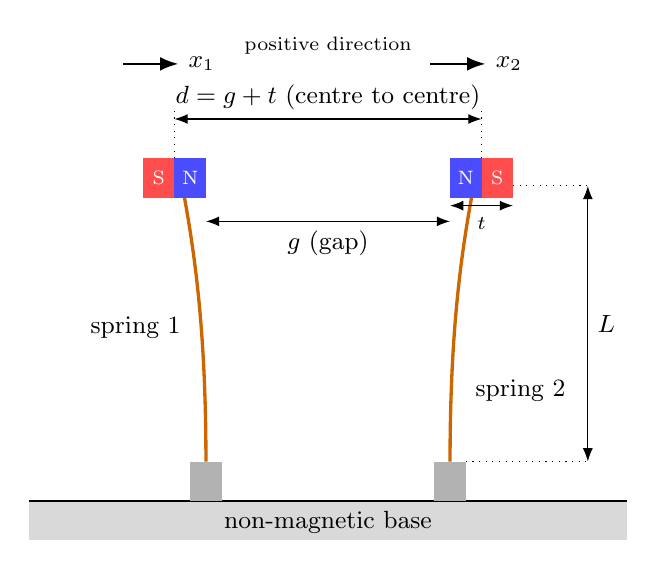
\begin{tikzpicture}[scale=1.0,>=Latex]
  % base
  \fill[gray!30] (-3.8,0) rectangle (3.8,-0.5);
  \draw[thick] (-3.8,0) -- (3.8,0);
  \node at (0,-0.27) {\small non-magnetic base};
  % clamps
  \fill[gray!60] (-1.75,0) rectangle (-1.35,0.5);
  \fill[gray!60] (1.35,0) rectangle (1.75,0.5);
  % springs (slightly bent outward)
  \draw[very thick,orange!80!black] (-1.55,0.5) .. controls (-1.55,2.2) and (-1.7,3.2) .. (-1.85,4.0);
  \draw[very thick,orange!80!black] (1.55,0.5) .. controls (1.55,2.2) and (1.7,3.2) .. (1.85,4.0);
  \node[font=\small,anchor=east] at (-1.75,2.2) {spring 1};
  \node[font=\small,anchor=west] at (1.75,1.4) {spring 2};
  % magnets (centres at x = -1.95 and +1.95)
  \fill[red!70] (-2.35,3.85) rectangle (-1.95,4.35);
  \fill[blue!70] (-1.95,3.85) rectangle (-1.55,4.35);
  \fill[blue!70] (1.55,3.85) rectangle (1.95,4.35);
  \fill[red!70] (1.95,3.85) rectangle (2.35,4.35);
  \node[white,font=\scriptsize] at (-2.15,4.1) {S};
  \node[white,font=\scriptsize] at (-1.75,4.1) {N};
  \node[white,font=\scriptsize] at (1.75,4.1) {N};
  \node[white,font=\scriptsize] at (2.15,4.1) {S};
  % gap g (between facing surfaces)
  \draw[<->] (-1.55,3.55) -- (1.55,3.55) node[midway,below,font=\small] {$g$ (gap)};
  % d (centre to centre) above
  \draw[dotted] (-1.95,4.35) -- (-1.95,5.0);
  \draw[dotted] (1.95,4.35) -- (1.95,5.0);
  \draw[<->] (-1.95,4.85) -- (1.95,4.85) node[midway,above,font=\small] {$d=g+t$ (centre to centre)};
  % magnet thickness t
  \draw[<->] (1.55,3.75) -- (2.35,3.75);
  \node[font=\scriptsize,anchor=north] at (1.95,3.72) {$t$};
  % displacement arrows x1, x2 (dashed positions)
  \draw[->,thick] (-2.6,5.55) -- (-1.9,5.55) node[right,font=\small] {$x_1$};
  \draw[->,thick] (1.3,5.55) -- (2.0,5.55) node[right,font=\small] {$x_2$};
  \node[font=\scriptsize,anchor=south] at (0,5.55) {positive direction};
  % L
  \draw[<->] (3.3,0.5) -- (3.3,4.0) node[midway,right,font=\small] {$L$};
  \draw[dotted] (1.75,0.5) -- (3.3,0.5);
  \draw[dotted] (2.35,4.0) -- (3.3,4.0);
\end{tikzpicture}
\caption{Coupled magnetic-mechanical oscillator. Both springs are slightly bent outwards by the static repulsion between the magnets. $d$ is the centre-to-centre separation of the magnets at equilibrium, $g$ is the surface-to-surface gap and $L$ is the free length of each spring. $x_1$ and $x_2$ are the horizontal displacements of the two magnets from their equilibrium positions, both taken positive in the same direction.}
\label{fig:setup_sketch}
\end{figure}

\subsection{Oscillation modes and frequencies}

If one spring is pulled aside and released, it does not simply oscillate at its own natural frequency. Its motion changes the distance between the magnets, which changes the repulsive force on the other spring, which therefore starts to move as well. Energy flows back and forth between the two springs, and the displacement of each spring shows the characteristic ``beats'' of a coupled system (Figure~\ref{fig:beats_example}).

The standard way to understand such motion is in terms of \emph{normal modes} \cite{taylor,french}: special patterns of motion in which every part of the system oscillates at the same single frequency. A system of two coupled oscillators has exactly two normal modes, and any motion whatsoever is a superposition of the two.

\begin{itemize}
\item \textbf{In-phase mode} (frequency $f_1$). The two magnets move together in the same direction by the same amount, so the separation between them never changes. The magnetic force stays constant at its equilibrium value and does no additional work; each spring simply oscillates at its own natural frequency as if the magnets were not there. This mode therefore ``does not see'' the coupling.
\item \textbf{Anti-phase mode} (frequency $f_2$). The two magnets move towards and away from each other. The separation, and with it the repulsive force, oscillates. The magnetic repulsion pushes each magnet back towards its equilibrium position whenever the magnets approach, so it acts as an extra restoring force in addition to the spring; the anti-phase mode is therefore stiffer and has the higher frequency, $f_2>f_1$.
\end{itemize}

\begin{figure}[htbp]
\centering
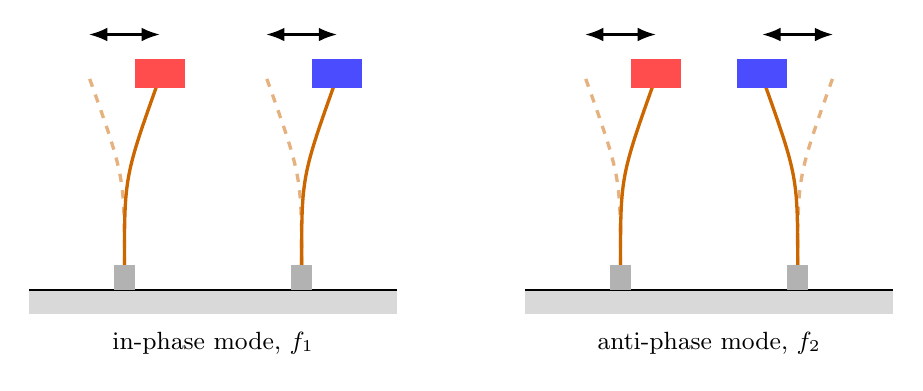
\begin{tikzpicture}[scale=0.9,>=Latex]
  \foreach \dx/\lab/\sgnA/\sgnB in {0/{in-phase mode, $f_1$}/1/1, 7/{anti-phase mode, $f_2$}/1/-1}{
    \begin{scope}[shift={(\dx,0)}]
      \fill[gray!30] (-2.6,0) rectangle (2.6,-0.35);
      \draw[thick] (-2.6,0) -- (2.6,0);
      \fill[gray!60] (-1.4,0) rectangle (-1.1,0.35);
      \fill[gray!60] (1.1,0) rectangle (1.4,0.35);
      \draw[very thick,orange!80!black] (-1.25,0.35) .. controls (-1.25,1.6) .. (-1.25+0.5*\sgnA,3.0);
      \draw[very thick,orange!80!black,dashed,opacity=0.5] (-1.25,0.35) .. controls (-1.25,1.6) .. (-1.25-0.5*\sgnA,3.0);
      \draw[very thick,orange!80!black] (1.25,0.35) .. controls (1.25,1.6) .. (1.25+0.5*\sgnB,3.0);
      \draw[very thick,orange!80!black,dashed,opacity=0.5] (1.25,0.35) .. controls (1.25,1.6) .. (1.25-0.5*\sgnB,3.0);
      \fill[red!70] (-1.25+0.5*\sgnA-0.35,2.85) rectangle (-1.25+0.5*\sgnA+0.35,3.25);
      \fill[blue!70] (1.25+0.5*\sgnB-0.35,2.85) rectangle (1.25+0.5*\sgnB+0.35,3.25);
      \draw[<->,thick] (-1.25-0.5,3.6) -- (-1.25+0.5,3.6);
      \draw[<->,thick] (1.25-0.5,3.6) -- (1.25+0.5,3.6);
      \node[font=\small] at (0,-0.75) {\lab};
    \end{scope}}
\end{tikzpicture}
\caption{The two normal modes. In the in-phase mode the separation of the magnets is constant, so the magnetic force plays no part and $f_1$ equals the natural frequency of a single spring. In the anti-phase mode the separation oscillates and the magnetic repulsion adds to the restoring force, so $f_2>f_1$.}
\label{fig:modes_sketch}
\end{figure}

When a single spring is displaced and released, both modes are set going at once, and the motion of each magnet is a mixture of the two. Because the two modes have slightly different frequencies they drift in and out of step: when they are in step the magnet swings widely, when they are out of step it almost stops. The displacement therefore shows a fast oscillation whose amplitude swells and shrinks periodically---the beats of Figure~\ref{fig:beats_example}. Two time scales can be read from such a trace: the period of the fast oscillation, which corresponds to the \emph{average frequency} $f_{\rm avg}=(f_1+f_2)/2$, and the time between successive swellings, the beat period $T_{\rm beat}$, whose reciprocal is the \emph{beat frequency} $f_{\rm beat}=f_2-f_1$. The proof of these two statements is given with the theory in Section~\ref{sec:modes} (equations~\eqref{eq:beats} and \eqref{eq:beats_identity}). Beats are the visible sign of coupling: the further apart the magnets, the weaker the coupling, the closer $f_2$ is to $f_1$, and the slower the beats, until with the magnets far apart each spring simply oscillates on its own.

\begin{figure}[htbp]
\centering
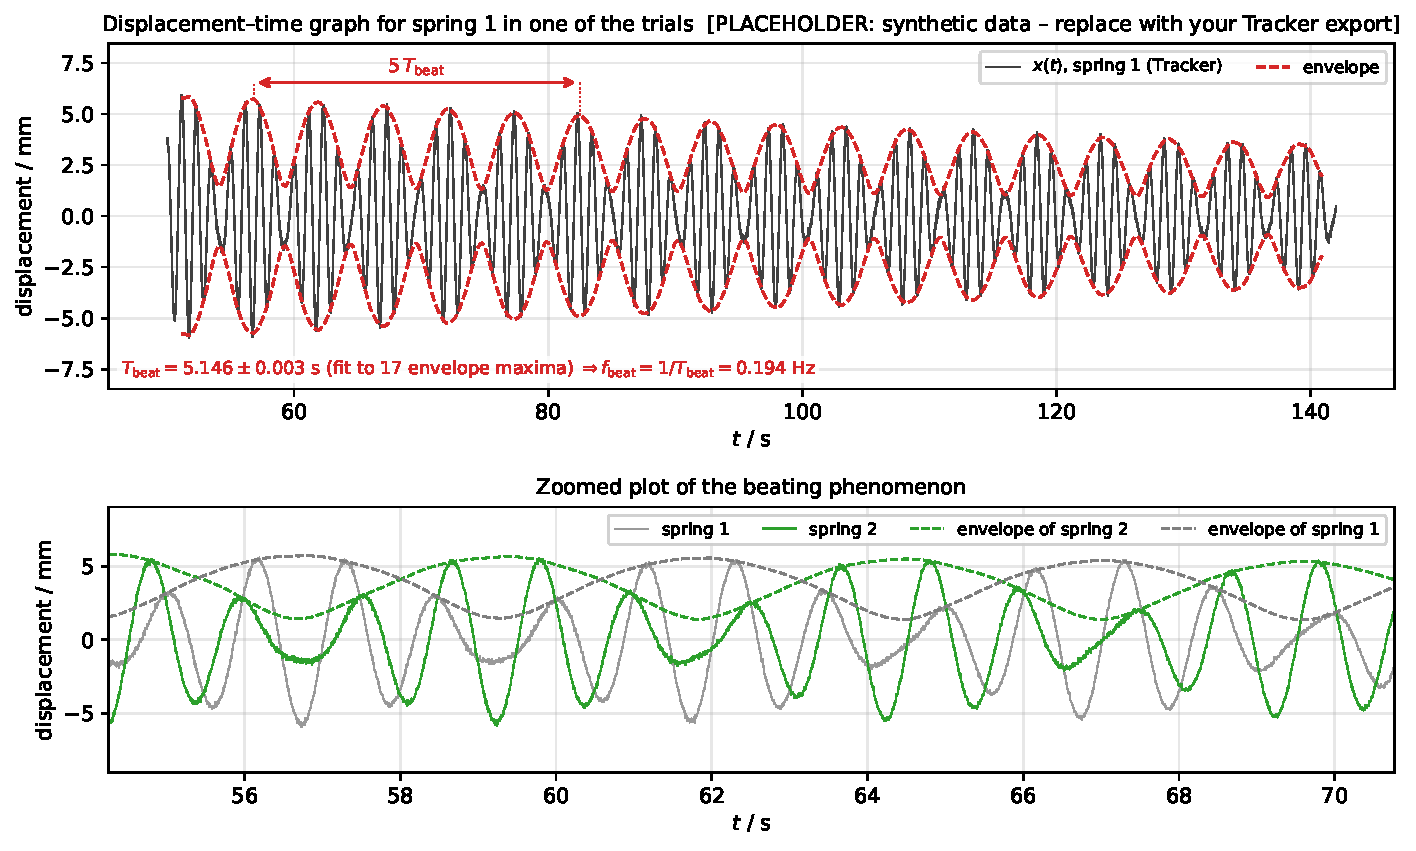
\includegraphics[width=\textwidth]{beats_measured_time}
\caption{Measured motion after spring~1 was displaced and released ($d=23\un{mm}$; Tracker, $240\un{fps}$). Top: displacement of spring~1. The amplitude of the fast oscillation swells and shrinks periodically (dashed envelope) because energy flows back and forth between the springs; the time between successive swellings is the beat period $T_{\rm beat}$. Bottom: three of these beats with both springs shown---spring~2 is at its largest amplitude whenever spring~1 is at its smallest. \TBM{Replace by \texttt{figs/beats\_measured\_time.pdf} produced with \texttt{plot\_beats.py --panels time}; state the trial and $d$ used.}}
\label{fig:beats_example}
\end{figure}

\subsection{Motivation and research question}

This experiment originates from problem~6, ``Magnetic-mechanical oscillator'', of the 2023 International Young Physicists' Tournament \cite{iypt}, which asks how the movement of two magnet-tipped leaf springs depends on relevant parameters. Of all the parameters, the separation of the magnets is the most interesting one, for two reasons. First, it is the parameter that controls the coupling, so it directly tests the physics of the normal modes described above. Second, the form of the dependence is a test of the law of force between two magnets: two small magnets facing each other are expected to behave as magnetic dipoles, whose mutual force falls as the inverse fourth power of their separation, and the extra stiffness of the anti-phase mode, which is the \emph{gradient} of that force, should fall as the inverse fifth power. Unlike a mechanical spring, whose stiffness is fixed once it is made, the magnetic ``spring'' has a stiffness that the experimenter can vary continuously by moving the clamps. A contactless, tunable coupling of this kind is also the principle behind magnetically coupled resonators used in wireless power transfer and in some sensors, which gives the investigation an application beyond the desk-top demonstration.

The research question is therefore:

\begin{keybox}
\textbf{How does the centre-to-centre separation $d$ of the magnets in a coupled magnetic-mechanical oscillator affect its two normal-mode frequencies $f_1$ and $f_2$, and hence its average frequency $f_{\mathrm{avg}}=(f_1+f_2)/2$ and beat frequency $f_{\mathrm{beat}}=f_2-f_1$?}
\end{keybox}

The first part of the question is answered by measuring $f_1$ and $f_2$ over a range of $d$. The second part follows from the first, because $f_{\rm avg}$ and $f_{\rm beat}$ are combinations of $f_1$ and $f_2$; they are reported because they are the two quantities that can be seen directly in a recording (Figure~\ref{fig:beats_example}). To turn the question into a quantitative test, the essay compares the measurements with a specific prediction: the point-dipole model of the magnets (Section~\ref{sec:theory}) predicts that the coupling term $f_2^2-f_1^2=2f_{\rm beat}f_{\rm avg}$ is proportional to $d^{-5}$.

Throughout the essay the separation $d$ is the \emph{centre-to-centre} distance between the two magnets at equilibrium, with both magnets mounted and the springs already bent outwards by the repulsion. If $g$ is the surface-to-surface gap between the facing poles and $t$ the thickness of each magnet, then $d=g+t$ (Figure~\ref{fig:setup_sketch}). The centre-to-centre distance is the natural variable of the dipole model, and defining $d$ at equilibrium (rather than as the distance between the clamps) removes the static bending of the springs from the problem: the equilibrium position, whatever it is, is simply where each oscillation is centred.

\section{Qualitative prediction}

Before any equations are written, the behaviour can be predicted qualitatively from the two facts established in the introduction.

\begin{enumerate}
\item In the in-phase mode the separation of the magnets does not change, so the magnetic force does not enter. Whatever $d$ is, $f_1$ should equal the natural frequency of a single spring carrying its magnet. \textbf{Prediction: $f_1$ is independent of $d$.}
\item In the anti-phase mode the magnetic repulsion acts as an extra spring. The stiffness of that extra spring is the rate at which the repulsive force changes with separation, $\gamma=-\dd F/\dd d$. The repulsion between two facing magnets weakens very rapidly with distance, faster than an inverse square, and its gradient weakens faster still. \textbf{Prediction: $f_2$ is largest when the magnets are close and falls towards $f_1$ as $d$ grows}; the beats slow down and eventually cannot be distinguished from a single oscillation.
\end{enumerate}

The difference between the two mode frequencies therefore measures the magnetic stiffness $\gamma$ alone, with the mechanical stiffness of the springs cancelling out. This is what makes the pair of frequencies such a clean probe of the magnetic force law.

\section{Hypothesis}

Modelling the two magnets as point magnetic dipoles (Section~\ref{sec:theory}) gives a repulsive force proportional to $d^{-4}$ and hence a magnetic stiffness $\gamma\propto d^{-5}$. Because the squared angular frequencies of the two modes differ by exactly $2\gamma/m$ (Section~\ref{sec:modes}), the hypothesis is:

\begin{keybox}
\begin{enumerate}[label=(\roman*)]
\item $f_1$ does not depend on $d$, so that $f_{\rm avg}$ and $f_{\rm beat}$ both approach constant values ($f_1$ and $0$ respectively) as $d$ increases;
\item $f_2^2-f_1^2=C\,d^{-5}$ with $C=\dfrac{3\muz\mum^2}{\pi^3 m}$, so that a graph of $\ln(f_2^2-f_1^2)$ against $\ln d$ is a straight line of gradient $-5$;
\item the intercept of that line, $\ln C$, agrees with the value calculated from the independently measured magnetic moment $\mum$ and effective mass $m$.
\end{enumerate}
\end{keybox}

Here $\muz=4\pi\times10^{-7}\un{T\,m\,A^{-1}}$ is the permeability of free space, $\mum$ is the magnetic dipole moment of each magnet and $m$ is the effective oscillating mass of one spring-plus-magnet.

\section{Variables}

\begin{description}[leftmargin=3.2cm,style=sameline]
\item[Independent] Centre-to-centre separation $d$ of the magnets at equilibrium, with both magnets mounted ($d=g+t$). Varied from $21\un{mm}$ to $60\un{mm}$ by moving one clamp along the base.
\item[Dependent] The two normal-mode frequencies $f_1$ and $f_2$, obtained from the Fourier spectrum of the recorded displacement $x_1(t)$; from them the average frequency $f_{\rm avg}=(f_1+f_2)/2$, the beat frequency $f_{\rm beat}=f_2-f_1$ and the coupling term $\Y\equiv f_2^2-f_1^2=2f_{\rm beat}f_{\rm avg}$, which is the quantity compared with the model.
\item[Controlled] The same pair of springs and the same pair of magnets throughout, in the same orientation; the clamped length $L$ of each spring (marked on the spring, clamp tightened to the same torque); the initial displacement (size and which spring is displaced); the release method (a card withdrawn horizontally); camera model, frame rate ($240\un{fps}$), resolution and distance from the apparatus; record length $T$; all settings of the analysis (tracking point, detrending, window, zero-padding).
\item[Uncontrolled / monitored] Room temperature (Young's modulus of copper and the remanence of the magnets both drift slightly with temperature, so all runs were done in one session); air currents (doors closed); residual slip in the clamps (checked by re-measuring $f_1$ at the start and end of the session).
\end{description}

\section{Theoretical model}\label{sec:theory}

The model is built in four steps: (1) each leaf spring with its magnet is reduced to a mass on a spring; (2) the repulsion between the magnets is written down using the point-dipole approximation; (3) the repulsion is linearised about the equilibrium separation, which turns it into a second spring that joins the two masses; (4) the resulting pair of coupled equations is solved for the two normal modes. The result is the tested relation, equation~\eqref{eq:main}. Full derivations of the standard results quoted in steps~1 and 2 are in Appendices~\ref{app:cantilever} and \ref{app:dipole}.

\subsection{The leaf spring as a mass on a spring}\label{sec:spring}

A leaf spring clamped at one end is a cantilever beam. For a beam of length $L$, width $b$, thickness $h$ and Young's modulus $E$, a transverse force $F$ applied at the free end produces a tip deflection \cite{gere}
\begin{equation}
x=\frac{FL^3}{3EI},\qquad I=\frac{bh^3}{12},
\end{equation}
where $I$ is the second moment of area of the rectangular cross-section (Appendix~\ref{app:cantilever}). The tip therefore behaves as a linear spring of stiffness
\begin{equation}
k=\frac{F}{x}=\frac{3EI}{L^3}=\frac{Ebh^3}{4L^3}.
\label{eq:k}
\end{equation}

The oscillating mass is not simply the magnet. The strip itself moves, but the parts near the clamp move much less than the tip. Rayleigh's method (Appendix~\ref{app:cantilever}) assumes that the strip vibrates in the shape of its static deflection curve and equates the kinetic energy of the strip to that of an equivalent point mass at the tip; the result is that a strip of mass $\mu L$ ($\mu$ = mass per unit length) contributes $\tfrac{33}{140}\mu L\approx0.236\,\mu L$ to the tip mass \cite{rao}. With a magnet (plus glue and any holder) of mass $M$ at the tip, the effective mass is
\begin{equation}
m=M+\tfrac{33}{140}\,\mu L,
\label{eq:meff}
\end{equation}
and the natural angular frequency of one spring is $\omega_0=\sqrt{k/m}$.

This lumped model replaces a continuous beam, which has infinitely many bending modes, by a single degree of freedom. It is accurate when the tip mass dominates: a numerical comparison with the full beam equation (Appendix~\ref{app:cantilever}) shows that the error in $f_2^2-f_1^2$ is below $1\,\%$ once $M\geq0.4\,\mu L$. Higher bending modes of the strip have frequencies at least $\sim 6$ times the fundamental and are easily separated in the spectrum.

\paragraph{Why calibrate dynamically as well as statically.} In principle $k$ and $m$ could be calculated from \eqref{eq:k} and \eqref{eq:meff}. In practice $E$ of a rolled copper strip is uncertain to $\sim10\,\%$ and $h^3$ amplifies the thickness uncertainty threefold, so the model is used only to understand the system while the constants are measured. Two measurements are made. (i) The \emph{ratio} $k/m$ of each spring is obtained by plucking the spring with its own magnet mounted and the other magnet removed; this gives the uncoupled frequencies $f_a$ and $f_b$ of the two springs directly and bypasses $E$, the Rayleigh factor and the lumped approximation altogether. (ii) The static stiffness $k$ is obtained from a load--deflection graph. The two together give $m=k/(2\pi f_a)^2$, which is needed for the \emph{absolute} test of the constant $C$ in equation~\eqref{eq:main}. The test of the \emph{exponent} $-5$ needs neither.

\subsection{Force between the two magnets}\label{sec:force}

A small permanent magnet of dipole moment $\mum$ produces, on its own axis at distance $r$ from its centre, a magnetic field parallel to the axis of magnitude \cite{griffiths}
\begin{equation}
B(r)=\frac{\muz}{4\pi}\,\frac{2\mum}{r^3}.
\label{eq:Baxis}
\end{equation}
A second dipole placed on that axis has potential energy $U=-\bm\mu\cdot\bm B$. When the two like poles face each other the second moment is anti-parallel to the field of the first, so $U=+\mum B(r)$ and the force on the second magnet is
\begin{equation}
F(r)=-\frac{\dd U}{\dd r}=-\mum\frac{\dd B}{\dd r}=\frac{\muz}{4\pi}\,\frac{6\mum^2}{r^4}
      =\frac{3\muz\mum^2}{2\pi r^4},
\label{eq:F}
\end{equation}
positive meaning repulsive (the full derivation, starting from the field of a dipole, is in Appendix~\ref{app:dipole}). The force falls as the \emph{fourth} power of the separation: a dipole field falls as $r^{-3}$ and the force is proportional to its gradient.

Equation~\eqref{eq:F} treats each magnet as a point dipole. This is exact only in the limit $r\gg D$, where $D$ is the size of the magnet. For the separations used here $r/D$ is only of order $2$--$6$ (Table~\ref{tab:constants}), so deviations are expected at the smallest separations; this is assumption~(a) in Section~\ref{sec:remarks} and is examined quantitatively in Section~\ref{sec:finite}.

\subsection{Equilibrium}\label{sec:equilibrium}

At rest the repulsion $F(d)$ bends each spring outwards by a static deflection $\delta$ given by $k\delta=F(d)$. If the clamps are set a distance $d_0$ apart, the magnets settle at $d=d_0+2\delta$, and finding $d$ from $d_0$ requires solving $k\,(d-d_0)/2=3\muz\mum^2/(2\pi d^4)$, a fifth-degree equation in $d$. This calculation is avoided entirely by \emph{measuring} $d$ at equilibrium with both magnets mounted, which is why $d$ was defined that way in Section~1.3. All displacements below are measured from this equilibrium.

\subsection{Linearised coupling and the normal modes}\label{sec:modes}

Let $x_1$ and $x_2$ be the horizontal displacements of the two magnets from their equilibrium positions, both positive in the same direction (Figure~\ref{fig:setup_sketch}). The separation of the magnets is then $r=d+x_2-x_1$. Consider magnet~1. Measured from the \emph{unstressed} position of the spring, its displacement is $x_1-\delta$, so the spring exerts $-k(x_1-\delta)$; the magnetic force on it is $-F(r)$ (it is pushed away from magnet~2, i.e.\ in the negative direction). Newton's second law gives
\begin{equation}
m\ddot x_1=-k(x_1-\delta)-F(d+x_2-x_1)=-kx_1+\big[F(d)-F(d+x_2-x_1)\big],
\end{equation}
where $k\delta=F(d)$ was used. The bracket is the \emph{change} of the magnetic force from its equilibrium value. For small displacements it is expanded to first order in $u=x_2-x_1$:
\begin{equation}
F(d+u)\approx F(d)+F'(d)\,u\quad\Rightarrow\quad F(d)-F(d+u)\approx-F'(d)\,u\equiv\gamma\,u ,
\end{equation}
where
\begin{equation}
\gamma\equiv-\frac{\dd F}{\dd r}\bigg|_{r=d}=\frac{4F(d)}{d}=\frac{6\muz\mum^2}{\pi d^5}
\label{eq:gamma}
\end{equation}
is the \emph{magnetic stiffness}: the extra restoring force per unit change of separation. It is positive because a repulsive force that weakens with distance always pushes the magnets back towards their equilibrium separation. The same steps for magnet~2 (on which the magnetic force is $+F(r)$) give the pair of linear equations
\begin{equation}
m\ddot x_1=-kx_1+\gamma(x_2-x_1),\qquad
m\ddot x_2=-kx_2-\gamma(x_2-x_1).
\label{eq:eom}
\end{equation}
These are exactly the equations of two equal masses on equal springs $k$ joined by a third spring of stiffness $\gamma$ \cite{taylor}; the magnetic field has become that third spring.

Equations~\eqref{eq:eom} are decoupled by adding and subtracting them. With the \emph{normal coordinates}
\begin{equation}
\eta\equiv x_1+x_2,\qquad \xi\equiv x_1-x_2,
\end{equation}
the sum of the two equations gives $m\ddot\eta=-k\eta$ and the difference gives $m\ddot\xi=-k\xi-2\gamma\xi$. Each normal coordinate therefore performs simple harmonic motion at its own angular frequency:
\begin{equation}
\boxed{\;\omega_1^2=\frac{k}{m},\qquad \omega_2^2=\frac{k+2\gamma}{m}\;}
\label{eq:modes}
\end{equation}
$\eta$ is the in-phase mode ($x_1=x_2$, $\xi=0$) and $\xi$ the anti-phase mode ($x_1=-x_2$, $\eta=0$), confirming the qualitative picture of Section~1.2. The factor 2 in $\omega_2^2$ arises because in the anti-phase mode a displacement $x_1=-x_2=\xi/2$ changes the separation by $\xi$, so each magnet feels the full $\gamma\xi$ while having moved only $\xi/2$. Equivalently, in matrix form $m\ddot{\bm x}=-\mathsf K\bm x$ with $\mathsf K=\begin{pmatrix}k+\gamma&-\gamma\\-\gamma&k+\gamma\end{pmatrix}$, whose eigenvalues are $k$ and $k+2\gamma$ with eigenvectors $(1,1)$ and $(1,-1)$.

Subtracting the two frequencies in \eqref{eq:modes} eliminates the spring stiffness $k$ altogether, and inserting \eqref{eq:gamma} gives the relation tested in this essay:
\begin{equation}
\boxed{\;f_2^2-f_1^2=\frac{\omega_2^2-\omega_1^2}{4\pi^2}=\frac{\gamma}{2\pi^2 m}
      =\frac{3\muz\mum^2}{\pi^3 m}\;d^{-5}\equiv C\,d^{-5}\;}
\label{eq:main}
\end{equation}
Taking natural logarithms,
\begin{equation}
\ln\!\big(f_2^2-f_1^2\big)=\ln C-5\ln d ,
\label{eq:lnln}
\end{equation}
a straight line of gradient $-5$ and intercept $\ln C$ in a graph of $\ln(f_2^2-f_1^2)$ against $\ln d$. The gradient tests the \emph{form} of the force law; the intercept tests its \emph{magnitude}, and can be compared with $C$ calculated from independently measured $\mum$ and $m$.

\paragraph{Motion after release; average and beat frequency.} The general motion is a superposition of the two modes, $\eta=\eta_0\cos(\omega_1t+\phi_1)$, $\xi=\xi_0\cos(\omega_2t+\phi_2)$; the frequencies are fixed by the system, the amplitudes $\eta_0$, $\xi_0$ by the way the motion is started. Both springs are released from rest, so $\phi_1=\phi_2=0$ and the mode amplitudes are simply the initial values of the normal coordinates, $\eta_0=x_1(0)+x_2(0)$ and $\xi_0=x_1(0)-x_2(0)$. Transforming back with $x_1=(\eta+\xi)/2$, $x_2=(\eta-\xi)/2$,
\begin{equation}
x_1(t)=\frac{\eta_0}{2}\cos\omega_1t+\frac{\xi_0}{2}\cos\omega_2t,\qquad
x_2(t)=\frac{\eta_0}{2}\cos\omega_1t-\frac{\xi_0}{2}\cos\omega_2t .
\label{eq:solution}
\end{equation}
Each displacement is the sum of two cosines at the two mode frequencies, so the Fourier spectrum of either spring contains two peaks, at $f_1$ and $f_2$, whose heights are in the ratio $\xi_0/\eta_0$. The \emph{positions} of the peaks do not depend on how the motion was started; this is the basis of the method of Section~\ref{sec:method}. The \emph{heights} do. For an idealised instantaneous release of spring~1, $x_1(0)=A$, $x_2(0)=0$, the two modes are excited equally ($\eta_0=\xi_0=A$) and the peaks are equal. In the experiment spring~1 is \emph{held} at $A$ before release, and while it is held the changed repulsion shifts spring~2 to a new rest position $x_2(0)=A\gamma/(k+\gamma)$ (from \eqref{eq:eom} with $\ddot x_2=0$), so that
\begin{equation}
\frac{\xi_0}{\eta_0}=\frac{A-x_2(0)}{A+x_2(0)}=\frac{k}{k+2\gamma}=\Big(\frac{f_1}{f_2}\Big)^2 ,
\label{eq:heights}
\end{equation}
about $0.65$ at $d=23\un{mm}$: the $f_2$ peak is expected to be lower than the $f_1$ peak, and the beats are not expected to reach zero amplitude (the envelope minimum is $x_2(0)$, not $0$). Both features are seen in Figure~\ref{fig:beats_example}; the observed height ratio, $\approx0.6$, agrees with \eqref{eq:heights} to within the non-linear correction discussed in Section~\ref{sec:nonlinear}.

For the equal-amplitude case the product-to-sum identity $\cos\alpha+\cos\beta=2\cos\frac{\alpha-\beta}{2}\cos\frac{\alpha+\beta}{2}$, with $\omega=2\pi f$, turns the first of \eqref{eq:solution} into
\begin{equation}
x_1(t)=A\cos\!\big(\pi(f_2-f_1)\,t\big)\,\cos\!\big(2\pi f_{\rm avg}\,t\big),\qquad f_{\rm avg}=\frac{f_1+f_2}{2},
\label{eq:beats}
\end{equation}
a fast oscillation at the average frequency $f_{\rm avg}$ whose amplitude $A\cos(\pi(f_2-f_1)t)$ varies slowly. The envelope cosine has frequency $(f_2-f_1)/2$, but what is observed is its \emph{modulus}, which reaches a maximum twice per cycle; the swellings of the trace therefore recur at
\begin{equation}
f_{\rm beat}=f_2-f_1=\frac{1}{T_{\rm beat}},
\qquad\text{and}\qquad
f_2^2-f_1^2=(f_2-f_1)(f_2+f_1)=2\,f_{\rm beat}\,f_{\rm avg}.
\label{eq:beats_identity}
\end{equation}
The same beat period holds for unequal amplitudes (the two cosines drift in and out of step once every $1/(f_2-f_1)$ whatever their sizes); only the depth of the minima changes. Equation~\eqref{eq:beats_identity} links the two quantities that can be read from a trace to the coupling term of \eqref{eq:main}: the beat frequency is the mode splitting itself, and $f_2^2-f_1^2$ is the product of the splitting and twice the average frequency. For spring~2 the same steps give $x_2=A\sin(\pi(f_2-f_1)t)\sin(2\pi f_{\rm avg}t)$: its envelope is a quarter of a beat period behind that of spring~1, so spring~2 is at full amplitude whenever spring~1 is momentarily at rest (Figure~\ref{fig:beats_example}, bottom), which is the energy transfer described qualitatively in the introduction. Finally, because each mode has the same amplitude in both springs (mode shapes $(1,1)$ and $(1,-1)$), the height ratio $\xi_0/\eta_0$ must be the \emph{same} in the spectra of the two springs whatever the starting condition, provided the springs are identical; a difference between the two ratios is a direct sign of non-identical springs (Section~\ref{sec:detuned}).

\subsection{Remarks and assumptions}\label{sec:remarks}

\paragraph{Units.} $[\muz\mum^2]=\mathrm{T\,m\,A^{-1}}\cdot\mathrm{A^2m^4}=\mathrm{T\,A\,m^5}$, and since $1\un{T}=1\un{kg\,A^{-1}s^{-2}}$ this is $\mathrm{kg\,m^5\,s^{-2}}$; dividing by $m$ (kg) and $d^5$ ($\mathrm{m^5}$) leaves $\mathrm{s^{-2}}$, the unit of $f^2$, as required. $C$ has units $\mathrm{m^5\,s^{-2}}$.

\paragraph{Magnitude of the coupling.} From \eqref{eq:modes}, $2\gamma/k=(f_2/f_1)^2-1$. With the values measured later ($f_2/f_1\approx1.29$ at $d=21\un{mm}$) this is about $0.67$, i.e.\ the magnetic ``spring'' is roughly one third as stiff as each leaf spring at the closest separation and about $0.02$ times as stiff at $40\un{mm}$. The static deflection follows from the same numbers: $\delta=F(d)/k=\gamma d/(4k)=\pi^2 (f_2^2-f_1^2)\,d/(2\omega_1^2)$, which is $\approx1.9\un{mm}$ at $21\un{mm}$ and $0.1\un{mm}$ at $40\un{mm}$. This is small compared with $d$ but not negligible compared with the uncertainty in $d$; it is one more reason to measure $d$ at equilibrium.

\paragraph{Predictions for the average and beat frequencies.} Combining \eqref{eq:main} with the definitions gives the two derived quantities named in the research question directly in terms of $d$:
\begin{equation}
f_{\rm beat}=\sqrt{f_1^2+Cd^{-5}}-f_1=\frac{Cd^{-5}}{2f_{\rm avg}},\qquad
f_{\rm avg}=\frac{f_1+\sqrt{f_1^2+Cd^{-5}}}{2}.
\label{eq:favg_fbeat}
\end{equation}
Since $f_{\rm avg}$ can only vary between $f_1$ (weak coupling) and $f_2/2+f_1/2$ (about $15\,\%$ higher at the closest separation used), while $d^{-5}$ varies by a factor of $25$, the beat frequency should fall almost as steeply as $d^{-5}$ itself and the beat period should lengthen roughly as $d^{5}$: from about $4\un{s}$ at $21\un{mm}$ to over $50\un{s}$ at $40\un{mm}$. The average frequency should be nearly constant, rising above $f_1$ only where the coupling is strong. In the weak-coupling limit $Cd^{-5}\ll f_1^2$ the square root can be expanded to give $f_{\rm beat}\approx Cd^{-5}/(2f_1)$, i.e.\ the beat frequency itself then follows the inverse-fifth-power law.

\paragraph{Assumptions.} The derivation assumed:
\begin{enumerate}[label=(\alph*)]
\item the magnets are point dipoles ($d\gg D$);
\item the displacements are small enough for the magnetic force to be linearised;
\item the two springs are identical ($k$ and $m$ the same for both);
\item each spring can be represented by a single lumped mass;
\item there is no damping;
\item the magnets stay coaxial (the tip of a bending cantilever actually tilts);
\item the FFT returns the true frequencies of the motion.
\end{enumerate}
Each of these is revisited in the evaluation (Section~\ref{sec:evaluation}), where its sign, size and remedy are estimated.

\section{Methodology}\label{sec:method}

\subsection{Background: measuring frequencies with the fast Fourier transform}\label{sec:fftbackground}

The frequencies $f_1$ and $f_2$ are extracted from the recorded displacement $x_1(t)$ by a discrete Fourier transform (DFT), computed with the fast Fourier transform (FFT) algorithm. Because every subsequent uncertainty estimate depends on how the DFT behaves, its relevant properties are set out here \cite{lyons,harris}.

\paragraph{Definition.} A record of $N$ samples $x_n=x(n\Delta t)$, $n=0,\dots,N-1$, taken at sampling frequency $f_s=1/\Delta t$ over a total time $T=N\Delta t$, is transformed into $N$ complex coefficients
\begin{equation}
X_k=\sum_{n=0}^{N-1}x_n\,e^{-2\pi i kn/N},\qquad k=0,\dots,N-1 .
\label{eq:dft}
\end{equation}
$|X_k|$ is the amplitude of the component at frequency $f_k=k/T$: coefficient $k$ corresponds to the sinusoid that completes exactly $k$ cycles in the record. Only $k\leq N/2$ carry independent information (frequencies up to the Nyquist frequency $f_s/2$). Here $f_s=240\un{Hz}$ is far above $2f_2\approx2\un{Hz}$, so aliasing is not an issue; the high frame rate is useful mainly because it gives many samples per cycle and hence low tracking noise per unit bandwidth.

\paragraph{Resolution.} The spectrum is evaluated only at the discrete frequencies $f_k=k/T$, spaced $1/T$ apart. For $T=30\un{s}$ the spacing (``bin width'') is $1/30\un{Hz}=\nbinT\un{mHz}$. Two sinusoids of frequencies $f_1$ and $f_2$ produce two separate maxima in $|X_k|$ only if their separation is at least of the order of one bin, $|f_2-f_1|\gtrsim1/T$; if they are closer, the two peaks merge into one. This is the fundamental ``uncertainty principle'' of spectral analysis: to separate two frequencies $\Delta f$ apart one must observe for at least $T\approx1/\Delta f$, i.e.\ long enough for the two oscillations to drift one full cycle out of step. In the language of beats, one must record at least one full beat period, $T\geq 1/(2 f_{\rm beat})=1/(f_2-f_1)$.

\paragraph{Leakage and windows.} The DFT implicitly assumes that the record repeats periodically. Unless a sinusoid completes a whole number of cycles in $T$, the repetition has a jump at the joins, and the energy of the sinusoid spreads (``leaks'') into neighbouring bins in a pattern determined by the Fourier transform of the record's rectangular boundary, a $\sin x/x$ shape with a main lobe two bins wide and side lobes only $13\un{dB}$ below the peak (Figure~\ref{fig:windows}). Multiplying the record by a smooth \emph{window} that tapers to zero at both ends (Hann, Blackman, \ldots) removes the jump and suppresses the side lobes, but at the price of a \emph{wider} main lobe: four bins for Hann, six for Blackman. Two tones must be separated by roughly the main-lobe half-width to be resolved, so the choice of window is a trade-off between resolution and leakage. For the present measurement the two peaks have similar heights and there is no strong interfering component, so the rectangular window (or the Hann window when its resolution suffices) is appropriate; this is the opposite of the usual ``always use a Hann window'' advice, which applies when weak components must be seen next to strong ones.

\begin{figure}[htbp]
\centering
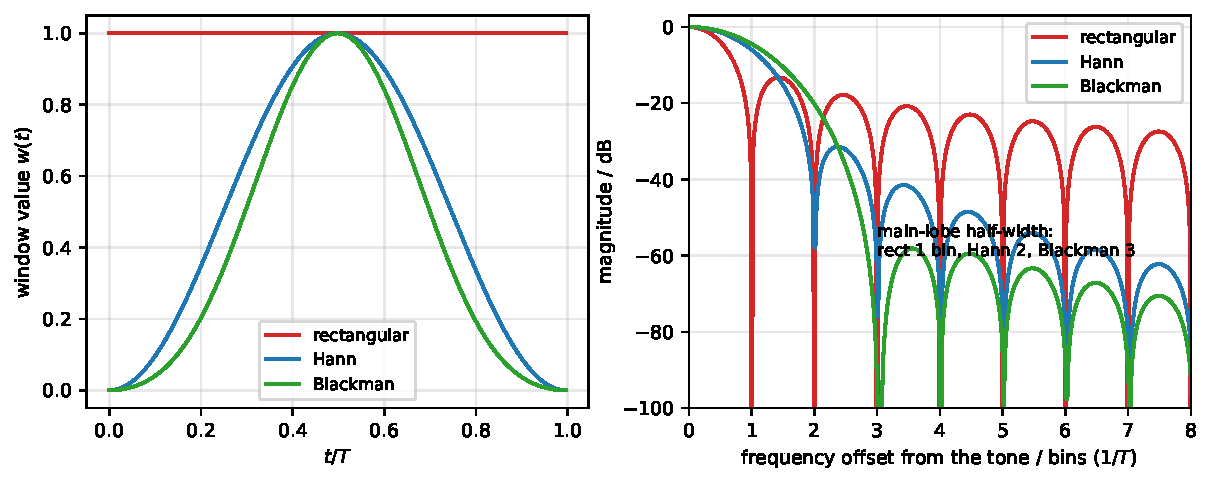
\includegraphics[width=\textwidth]{F_windows}
\caption{Left: the three window functions. Right: their spectra in units of the bin width $1/T$. The rectangular window has the narrowest main lobe (best resolution) but the highest side lobes (most leakage); Hann and Blackman suppress leakage at the cost of doubling and tripling the main-lobe width.}
\label{fig:windows}
\end{figure}

\begin{figure}[htbp]
\centering
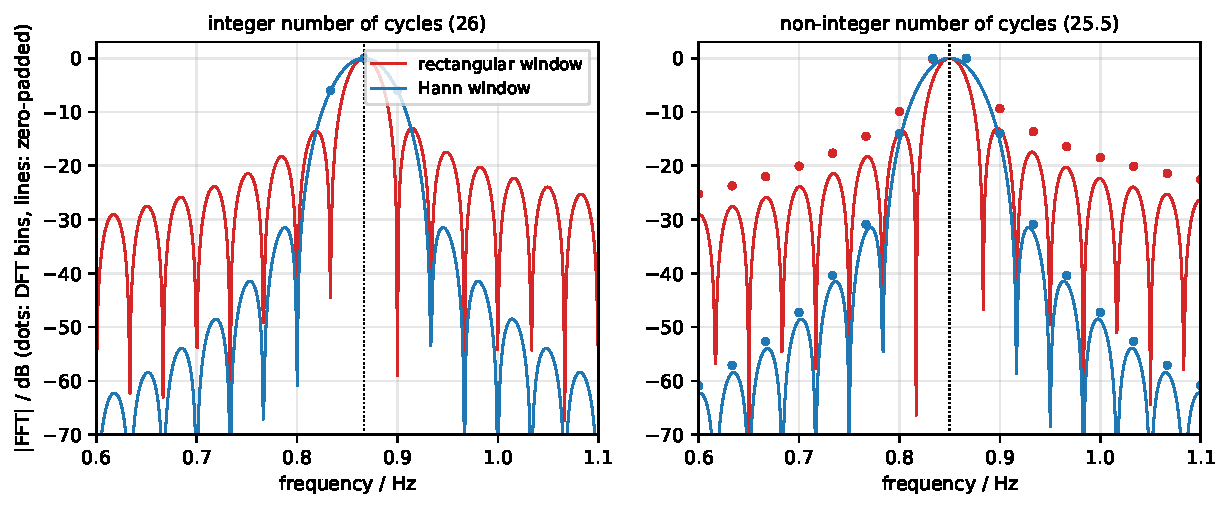
\includegraphics[width=\textwidth]{F_leakage}
\caption{Leakage for a single $0.85$--$0.87\un{Hz}$ tone recorded for $30\un{s}$ at $240\un{fps}$. Left: the tone completes exactly 26 cycles, so with a rectangular window all the energy falls in one bin (red dot). Right: $25.5$ cycles; the rectangular window spreads energy into many bins (red dots), the Hann window (blue) confines it to a few. Lines show the zero-padded (interpolated) spectra.}
\label{fig:leakage}
\end{figure}

\paragraph{Zero-padding and peak interpolation.} Appending zeros to the record before the FFT evaluates the same underlying spectrum at more closely spaced frequencies. It does \emph{not} improve the resolution (the main-lobe width is set by $T$), but it locates the maximum of an isolated peak more precisely than the nearest bin. In this essay every spectrum is zero-padded to $2^{20}$ points, and the peak position is refined by fitting a parabola through the three highest points, so the bin-centring error $\pm1/(2T)$ that would otherwise apply is removed.

\paragraph{Peak pulling.} When two peaks are close enough that their main lobes overlap, each maximum is displaced by the tail of the other: the peaks are pushed apart (or, for some phase differences, pulled together). This bias, not the random noise, turns out to be the dominant error at the larger separations, and it is quantified in Section~\ref{sec:fftres}.

\paragraph{Damping linewidth.} A decaying oscillation $e^{-t/\tau}\cos2\pi ft$ recorded for $T\gg\tau$ has a Lorentzian amplitude spectrum whose full width at half maximum is $\sqrt3/(\pi\tau)$ (the more often quoted $1/(\pi\tau)$ is the width of the \emph{power} spectrum). For the observed decay time $\tau\approx25\un{s}$ this is $\nlwAmp\un{Hz}$: a floor on the resolution that no record length can remove, comparable to $f_2-f_1$ at $d\geq35\un{mm}$.

\paragraph{Pre-processing.} The tracked coordinate contains a large constant offset (the pixel coordinate of the equilibrium position, typically $50$ times the oscillation amplitude) and possibly a slow drift. A constant is a zero-frequency component; with a rectangular window its leakage at $\approx16$ bins from zero (where $f_1\approx0.8\un{Hz}$ sits at $T=20\un{s}$) is only $\sim34\un{dB}$ down, comparable to the signal peaks. The mean and any linear trend are therefore subtracted (``detrending'') before the transform. Video frames are not perfectly uniformly spaced; the time stamps are checked and the data resampled to a uniform grid by linear interpolation if the timing jitter exceeds $1\,\%$ of a frame.

\subsection{Set-up and apparatus}

\begin{figure}[htbp]
\centering
\fbox{\parbox[c][6.5cm][c]{0.85\textwidth}{\centering\TBM{Insert labelled photograph of the actual apparatus: base, clamps, springs, magnets, scale bar in the plane of motion, camera position. Label $d$, $L$ and the tracked point.}}}
\caption{Photograph of the apparatus. \TBM{to be inserted}}
\label{fig:photo}
\end{figure}

\begin{table}[htbp]
\centering\small
\caption{Apparatus.}
\label{tab:apparatus}
\begin{tabular}{@{}p{4.2cm}p{10.5cm}@{}}
\toprule
Item & Specification \\
\midrule
Leaf springs (2) & copper strip, free length $L=\TBM{\ldots}\un{mm}$, width $b=\TBM{\ldots}\un{mm}$, thickness $h=\TBM{\ldots}\un{mm}$\\
Magnets (2) & NdFeB, \TBM{shape, $D\times t$}, mass $M=\TBM{\ldots}\un{g}$, grade \TBM{N\ldots}\\
Base and clamps & aluminium/wooden base with two sliding aluminium clamps; brass screws (non-magnetic)\\
Camera & smartphone in slow-motion mode, $240\un{fps}$, $1080\times1920$ pixels, on a tripod $\approx\TBM{\ldots}\un{m}$ from the apparatus, optical axis perpendicular to the plane of motion\\
Scale & steel rule with $1\un{mm}$ divisions placed in the plane of motion for calibration; digital calliper ($\pm0.02\un{mm}$) for $g$, $t$, $b$, $h$\\
Balance & electronic balance, resolution $0.01\un{g}$, for $M$, $\mu$ and the magnetic-force measurement\\
Masses & slotted masses $1$--$20\un{g}$ for the static stiffness measurement\\
Software & Tracker 6 (video analysis) \cite{tracker}; Python 3 with NumPy/SciPy for FFT, fitting and simulation (Appendix~\ref{app:code})\\
\bottomrule
\end{tabular}
\end{table}

\subsection{Method of data collection}

\paragraph{First attempt: reading the beat period.} The natural first approach, used in many coupled-pendulum experiments, is to read the average period and the beat period directly from the recorded $x_1(t)$ and use equation~\eqref{eq:beats_identity}. This worked at the smallest separations, where several beats fit into one record, but failed beyond about $30\un{mm}$: the beat period becomes longer than $10\un{s}$, fewer than three envelope minima fit into the record, the envelope minima are shallow and their positions cannot be read to better than a quarter of a cycle. It also breaks down completely once the beat period exceeds the decay time of the oscillation.

\paragraph{Adopted method: FFT of the displacement.} The recorded displacement is transformed as described in Section~\ref{sec:fftbackground} and the two mode frequencies are read as the positions of the two highest peaks (Figure~\ref{fig:tracker}). This uses the whole record rather than a few envelope minima, gives both frequencies directly, and its limitations (resolution, leakage, pulling) can be quantified. It is the method used for all the data in Section~\ref{sec:rawdata}.

\begin{figure}[htbp]
\centering
\fbox{\parbox[c][5.5cm][c]{0.85\textwidth}{\centering\TBM{Insert a screenshot of Tracker with the tracked point on the magnet, the measured $x_1(t)$ for one run (e.g.\ $d=25\un{mm}$) and its FFT with $f_1$ and $f_2$ labelled. (Figure~\ref{fig:beats_example} shows the trace of one run; here the spectrum should be shown as well, e.g.\ with \texttt{plot\_beats.py --panels fft}.)}}}
\caption{Measured displacement $x_1(t)$ and its amplitude spectrum for one trial. \TBM{to be inserted}}
\label{fig:tracker}
\end{figure}

\subsection{Procedures}

\subsubsection{Static stiffness \texorpdfstring{$k$}{k} of each spring}
\begin{enumerate}
\item Clamp the spring horizontally with the same free length $L$ as in the oscillation experiment, with a mm scale behind the tip.
\item Hang slotted masses $m_i=1,2,\ldots,10\un{g}$ from the tip with a light loop of thread; record the tip deflection $x_i$ for each load, loading and unloading.
\item Plot $F_i=m_ig$ against $x_i$; the gradient of the best-fit line through the origin is $k$. The straightness of the graph also checks that the spring is linear over the range of deflections used ($\pm12\un{mm}$).
\end{enumerate}

\subsubsection{Uncoupled frequencies \texorpdfstring{$f_a$, $f_b$}{fa, fb} of each spring (dynamic calibration)}
\begin{enumerate}
\item With only spring~1 (and its own magnet) mounted, displace it by $3\un{mm}$, release, and record $60\un{s}$ of video.
\item Track the magnet and take the FFT; the single peak is $f_a$. Repeat three times.
\item Repeat for spring~2 alone to obtain $f_b$. The difference $f_b-f_a$ measures how far assumption~(c) (identical springs) is from the truth and is used in Section~\ref{sec:detuned}.
\end{enumerate}

\subsubsection{Magnetic moment \texorpdfstring{$\mum$}{mu\_m}}
\begin{enumerate}
\item Fix one magnet on the pan of the electronic balance (on a non-magnetic spacer) and tare.
\item Hold the second magnet coaxially above it, like poles facing, on a non-magnetic stand whose height is set with a calliper; record the apparent mass change $\Delta m$ at 6 separations $r$ between $20$ and $40\un{mm}$.
\item $F=\Delta m\,g$. Plot $\ln F$ against $\ln r$: the gradient tests the $r^{-4}$ law directly (independent of any oscillation) and the intercept gives $\mum$ through equation~\eqref{eq:F}. Compare with the datasheet value $\mum=B_rV/\muz$, where $B_r$ is the remanence and $V$ the volume of the magnet.
\end{enumerate}

\subsubsection{Masses}
Weigh each magnet (with its glue/holder) to obtain $M$, and weigh a measured length of the same copper strip to obtain $\mu$; hence $m$ from equation~\eqref{eq:meff} as a cross-check on $m=k/(2\pi f_a)^2$.

\subsubsection{Mode frequencies against separation}\label{sec:mainproc}
\begin{enumerate}
\item Mount both springs. Slide clamp~2 until the centre-to-centre separation of the magnets, read from a calibrated video frame with the system at rest, is the required $d$ (checked as $g+t$ with the calliper; $\pm0.5\un{mm}$ because of the outward bending). Values used: $d=21,23,25,28,31,35,40,45,50,60\un{mm}$.
\item Displace spring~1 by $A=10\un{mm}$ using a card held against the magnet, with spring~2 at rest; withdraw the card horizontally to release.
\item Record $30\un{s}$ at $240\un{fps}$. Repeat three times at each $d$.
\item In Tracker, calibrate the scale, define the $x$ axis along the line joining the magnets and auto-track the centre of magnet~1. Export $t$, $x_1$.
\item Detrend, apply the window, zero-pad to $2^{20}$ points, compute the amplitude spectrum, and read the two highest peaks with parabolic interpolation. Record $f_1$ (lower) and $f_2$ (higher). If only one peak is present, record ``unresolved''.
\end{enumerate}

\paragraph{Safety.} Neodymium magnets pinch strongly and shatter if allowed to snap together; they were handled one at a time and kept away from the phone, cards and the balance's electronics when not in use. The spring tips were not sharp, but eye protection was worn while the springs were plucked.

\section{Raw data}\label{sec:rawdata}

\subsection{Constants of the apparatus}

\begin{table}[htbp]
\centering\footnotesize
\caption{Constants of the apparatus. Values in red are still to be measured (Section~\ref{sec:method}).}
\label{tab:constants}
\setlength{\tabcolsep}{4pt}
\begin{tabular}{@{}p{4.3cm}cp{4.6cm}p{3.6cm}@{}}
\toprule
Quantity & Symbol & Value & Source \\
\midrule
Free length of spring & $L$ & \TBM{\ldots}$\pm0.5\un{mm}$ & rule \\
Width, thickness of strip & $b$, $h$ & \TBM{\ldots}, \TBM{\ldots}$\un{mm}$ ($\pm0.02$) & calliper (mean of 5) \\
Mass per unit length & $\mu$ & \TBM{\ldots}$\un{g\,m^{-1}}$ & balance, 300 mm of strip \\
Magnet diameter, thickness & $D$, $t$ & \TBM{\ldots}, \TBM{\ldots}$\un{mm}$ & calliper \\
Magnet mass (with holder) & $M$ & \TBM{\ldots}$\pm0.01\un{g}$ & balance \\
Static stiffness, spring 1 / 2 & $k$ & \TBM{\ldots} / \TBM{\ldots}$\un{N\,m^{-1}}$ & load--deflection graph \\
Uncoupled frequency, spring 1 / 2 & $f_a$ / $f_b$ & \TBM{\ldots} / \TBM{\ldots}$\un{Hz}$ ($\pm0.003$) & FFT, 60 s, 3 trials \\
Effective mass & $m=k/(2\pi f_a)^2$ & \TBM{\ldots}$\un{g}$ & derived \\
Magnetic moment & $\mum$ & \TBM{\ldots}$\un{A\,m^2}$ & balance method / datasheet \\
Predicted constant & $C=3\muz\mum^2/(\pi^3m)$ & \TBM{\ldots}$\un{m^5\,s^{-2}}$ & derived \\
Decay time of oscillation & $\tau$ & $\approx25\un{s}$ & envelope of $x_1(t)$ \\
Frame rate, record length & $f_s$, $T$ & $240\un{fps}$, $30\un{s}$ ($N=\nNsamples$) & camera metadata \\
\bottomrule
\end{tabular}
\end{table}

\begin{table}[htbp]
\centering\small
\caption{Static load--deflection data for spring 1 (spring 2 in Appendix~\ref{app:rawdata}). \TBM{to be measured}}
\label{tab:static}
\begin{tabular}{@{}cccccc@{}}
\toprule
load / g & $F$ / mN & $x$ (loading) / mm & $x$ (unloading) / mm & mean $x$ / mm & $\Delta x$ / mm\\
\midrule
1 & 9.8 & \TBM{} & \TBM{} & \TBM{} & 0.5\\
2 & 19.6 & & & & \\
$\vdots$ & & & & & \\
10 & 98.1 & & & & \\
\bottomrule
\end{tabular}
\end{table}

\subsection{Mode frequencies}

Table~\ref{tab:rawfreq} lists the two peak frequencies read from the spectrum of each trial. All spectra were computed from $T=30\un{s}$ records sampled at $f_s=240\un{Hz}$ ($N=\nNsamples$ samples), detrended, with a rectangular window, zero-padded to $2^{20}$ points and with parabolic peak interpolation; the bin width is $1/T=\nbinT\un{mHz}$. The uncertainty of each mean is taken as the half-range of the three trials (three trials are too few for a meaningful standard deviation) or the resolution-limited value $\pm5\un{mHz}$ (Section~\ref{sec:fftres}), whichever is larger. The last column states whether the two peaks were resolved, using the criterion $f_2-f_1\geq2/T=67\un{mHz}$ for a clean separation with a rectangular window; the cases $35$ and $40\un{mm}$ are marked as \emph{marginal}, and at $45$, $50$ and $60\un{mm}$ only a single peak was present. The unresolved rows are a result in themselves (they mark where the beat period exceeds the record length) rather than missing data.

\begin{table}[htbp]
\centering\footnotesize
\caption{Peak frequencies read from the FFT of $x_1(t)$ for each trial ($A=10\un{mm}$, $T=30\un{s}$, $240\un{fps}$, rectangular window). The trial columns are to be filled from the raw exports; the means are the values used in the analysis.}
\label{tab:rawfreq}
\setlength{\tabcolsep}{3.5pt}
\begin{tabular}{@{}c ccc c ccc c c@{}}
\toprule
$d\pm0.5$ & \multicolumn{3}{c}{$f_1$ / Hz} & mean $f_1$ & \multicolumn{3}{c}{$f_2$ / Hz} & mean $f_2$ & resolved?\\
/ mm & tr.\,1 & tr.\,2 & tr.\,3 & $\pm0.005$ & tr.\,1 & tr.\,2 & tr.\,3 & $\pm0.005$ & ($f_2-f_1\geq2/T$)\\
\midrule
21 & \TBM{} & \TBM{} & \TBM{} & 0.823 & \TBM{} & \TBM{} & \TBM{} & 1.063 & yes\\
23 & & & & 0.808 & & & & 1.005 & yes\\
25 & & & & 0.812 & & & & 0.953 & yes\\
28 & & & & 0.810 & & & & 0.907 & yes\\
31 & & & & 0.807 & & & & 0.881 & yes\\
35 & & & & 0.806 & & & & 0.845 & marginal (1.2 bins)\\
40 & & & & 0.802 & & & & 0.811 & no (0.3 bins)\\
45 & & & & \multicolumn{5}{c}{single peak at $\approx0.80\un{Hz}$} & no\\
50 & & & & \multicolumn{5}{c}{single peak at $\approx0.80\un{Hz}$} & no\\
60 & & & & \multicolumn{5}{c}{single peak at $\approx0.80\un{Hz}$} & no\\
\bottomrule
\end{tabular}
\end{table}

\paragraph{Qualitative observations.} At $21$--$25\un{mm}$ the beats were obvious to the eye, with the energy passing completely from one spring to the other and back within a few seconds. At $35\un{mm}$ one beat took roughly $25\un{s}$, comparable to the time for the amplitude to decay by a factor $e$, and by $45\un{mm}$ the second spring barely moved during the whole record. A small amount of motion perpendicular to the line joining the magnets was visible when the release was not perfectly horizontal; those trials were repeated. The displacement traces also showed that the oscillation frequency of the anti-phase motion was slightly higher during the first few seconds (largest amplitude) than later, an observation that becomes important in Section~\ref{sec:nonlinear}.

\section{Analysis}\label{sec:analysis}

\subsection{Processed data and uncertainty propagation}

For each separation the coupling term $\Y=f_2^2-f_1^2$ and its logarithm are computed together with $\ln d$ and $d^{-5}$. The uncertainties follow from the standard rules for propagating independent uncertainties \cite{taylorerr}: for a power, $\Delta(f^2)=2f\,\Delta f$; for a difference, the absolute uncertainties add; for a logarithm, $\Delta(\ln q)=\Delta q/q$. Hence
\begin{equation}
\Delta\Y=2f_1\Delta f_1+2f_2\Delta f_2,\qquad
\Delta(\ln\Y)=\frac{\Delta\Y}{\Y},\qquad
\Delta(\ln d)=\frac{\Delta d}{d},\qquad
\Delta\big(d^{-5}\big)=5\,\frac{\Delta d}{d}\,d^{-5}.
\label{eq:unc}
\end{equation}

\paragraph{Sample calculation ($d=25\un{mm}$).}
$\Y=0.953^2-0.812^2=0.9082-0.6593=0.2489\un{Hz^2}$;\;
$\Delta\Y=2(0.812)(0.005)+2(0.953)(0.005)=0.0176\un{Hz^2}$ ($7.1\,\%$);\;
$\ln\Y=-1.391\pm0.071$;\;
$\ln(d/\mathrm{mm})=\ln25=3.219$, $\Delta(\ln d)=0.5/25=0.020$;\;
$d^{-5}=(0.025\un{m})^{-5}=1.024\times10^{8}\un{m^{-5}}$, $\Delta(d^{-5})=5(0.020)(1.024\times10^8)=0.10\times10^8\un{m^{-5}}$.

Two features of Table~\ref{tab:processed} deserve comment before any graph is drawn. First, although every frequency has the same uncertainty ($\pm5\un{mHz}$), the uncertainty of $\ln\Y$ grows from $0.04$ at $21\un{mm}$ to $0.26$ at $35\un{mm}$ and $1.1$ at $40\un{mm}$, because $\Y$ is a small difference of two nearly equal squares. The points are far from equally reliable, and a fitting procedure that treats them equally will be dominated by the least reliable ones. Second, the horizontal uncertainty $\Delta(\ln d)=\Delta d/d$ is $0.024$ at $21\un{mm}$, comparable to the vertical uncertainty there; in a $d^{-5}$ law a $2.4\,\%$ error in $d$ becomes a $12\,\%$ error in $\Y$. Error bars must therefore be drawn on both axes.

\begin{table}[htbp]
\centering\footnotesize
\caption{Processed data. $\Delta f_1=\Delta f_2=0.005\un{Hz}$, $\Delta d=0.5\un{mm}$. The $40\un{mm}$ row is shown for completeness but is excluded from the fits because its peaks were not resolved (Table~\ref{tab:rawfreq}).}
\label{tab:processed}
\setlength{\tabcolsep}{3.2pt}
\begin{tabular}{@{}c cc cc cc cc cc@{}}
\toprule
$d$/mm & $\ln\frac{d}{\mathrm{mm}}$ & $\Delta$ & $f_1$/Hz & $f_2$/Hz & $\Y$/Hz$^2$ & $\Delta\Y$ & $\ln\frac{\Y}{\mathrm{Hz^2}}$ & $\Delta$ & $\frac{d^{-5}}{10^8\,\mathrm{m^{-5}}}$ & $\Delta$\\
\midrule
\tabinput{tables/tab_processed}
\bottomrule
\end{tabular}
\end{table}

\subsection{Graph 1: \texorpdfstring{$\ln(f_2^2-f_1^2)$}{ln(f2²−f1²)} against \texorpdfstring{$\ln d$}{ln d}}

Figure~\ref{fig:G1} is the main graph of the essay. The six resolved points ($21$--$35\un{mm}$) lie close to a straight line, confirming a power law, but the line is clearly \emph{less steep} than the dipole prediction. An unweighted least-squares fit (Excel's LINEST; Appendix~\ref{app:uncertainty} gives the formulae) returns
\begin{equation}
\text{gradient}=\ngradSix\pm\ngradSixErr,\qquad \text{intercept}=\nintSix\pm0.64,\qquad R^2=0.989 .
\end{equation}
The best/worst-line method, drawing the steepest and shallowest lines compatible with the error bars of the end points, gives gradients between $\ngradSteep$ and $\ngradShallow$, a somewhat wider range than the statistical one because it uses only two points. A fit that weights each point by $1/[\Delta(\ln\Y)]^2$, so that the precise small-$d$ points count more, gives $\ngradW\pm\ngradWErr$. Whichever way it is done, the measured exponent is between $-3.5$ and $-3.8$, and the predicted value $-5$ lies $5$--$6$ standard errors away. If the unresolved $40\un{mm}$ point is (wrongly) included, the gradient becomes $\ngradSeven$; this shows how strongly a single point with a $\pm1.1$ error bar in $\ln\Y$ can swing an unweighted fit, and is the reason it is excluded.

\begin{figure}[htbp]
\centering
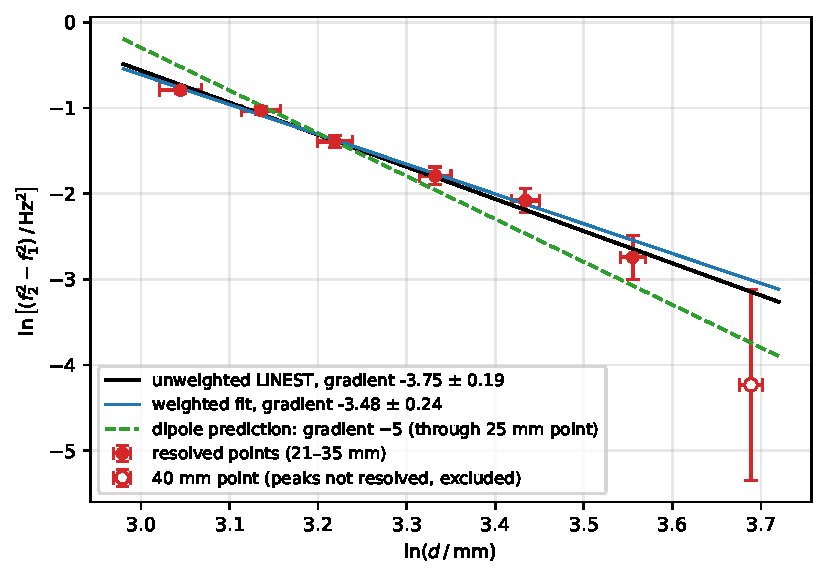
\includegraphics[width=0.9\textwidth]{G1_lnln}
\caption{Graph 1: $\ln(f_2^2-f_1^2)$ against $\ln d$ with uncertainties on both axes (equation~\eqref{eq:unc}). The unweighted line has gradient $\ngradSix\pm\ngradSixErr$; the weighted line $\ngradW\pm\ngradWErr$; the dashed green line is the dipole prediction of gradient $-5$, drawn through the $25\un{mm}$ point. The open symbol is the $40\un{mm}$ point, whose peaks were not resolved.}
\label{fig:G1}
\end{figure}

\subsection{Graph 2: \texorpdfstring{$f_2^2-f_1^2$}{f2²−f1²} against \texorpdfstring{$d^{-5}$}{d⁻⁵}}

Equation~\eqref{eq:main} can also be tested without logarithms by plotting $\Y$ against $d^{-5}$, where it predicts a straight line through the origin of gradient $C$ (Figure~\ref{fig:G2}). The line of best fit through the origin has gradient
\begin{equation}
C_{\rm exp}=(2.08\pm0.15)\times10^{-9}\un{m^5\,s^{-2}},
\end{equation}
but the points do not lie on it: the small-$d^{-5}$ points (large $d$) fall above the line and the large-$d^{-5}$ points below, and a line with a free intercept fits much better, with intercept $0.06\un{Hz^2}$. A positive intercept means that $\Y$ does not tend to zero as $d\to\infty$ as fast as $d^{-5}$ does, the same information as the too-shallow gradient of Graph~1 seen from a different angle. The linear plot is the better graph for judging the magnitude $C$ because it does not distort the error bars, while the logarithmic plot is the better one for judging the exponent.

\begin{figure}[htbp]
\centering
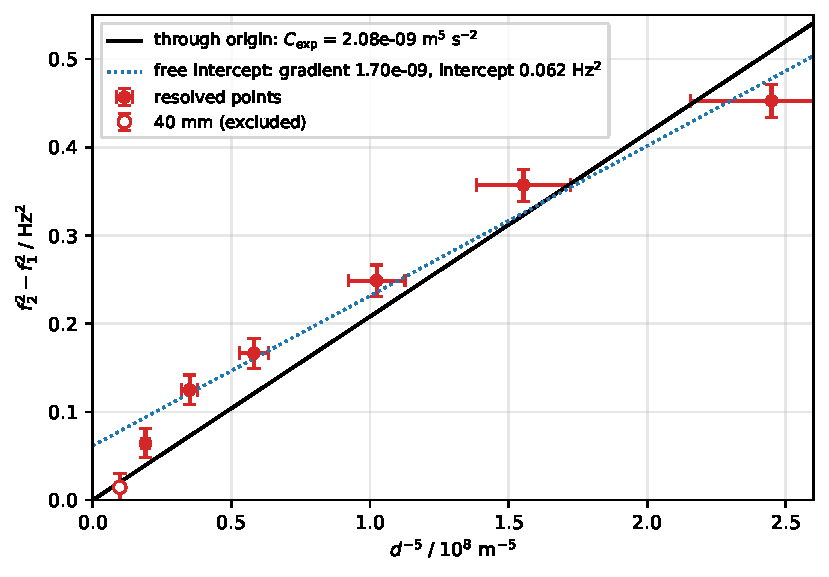
\includegraphics[width=0.9\textwidth]{G2_Y_vs_d5}
\caption{Graph 2: $f_2^2-f_1^2$ against $d^{-5}$. The dipole model predicts a straight line through the origin. The systematic curvature of the points about the through-origin line is the counterpart of the shallow gradient in Graph 1.}
\label{fig:G2}
\end{figure}

\subsection{Graph 3: the individual frequencies}

Figure~\ref{fig:G3} shows $f_1$ and $f_2$ separately. $f_2$ falls steeply towards $f_1$ as predicted. $f_1$, which the model says should be constant, is \emph{not} quite constant: it decreases from $0.823\un{Hz}$ at $21\un{mm}$ to $0.802\un{Hz}$ at $40\un{mm}$, a drift of $2.6\,\%$, or about $4$ times its uncertainty; a straight line through $f_1$ has gradient $(\nfOneSlope\pm0.4)\un{mHz\,mm^{-1}}$. The right-hand panel shows the residuals of the six resolved points from the Graph-1 line. Their signs, $-,+,-,+,+,-$, and their magnitudes, which are not much larger than the error bars, suggest a slight concave-down curvature rather than random scatter, although with six points this cannot be established firmly.

\begin{figure}[htbp]
\centering
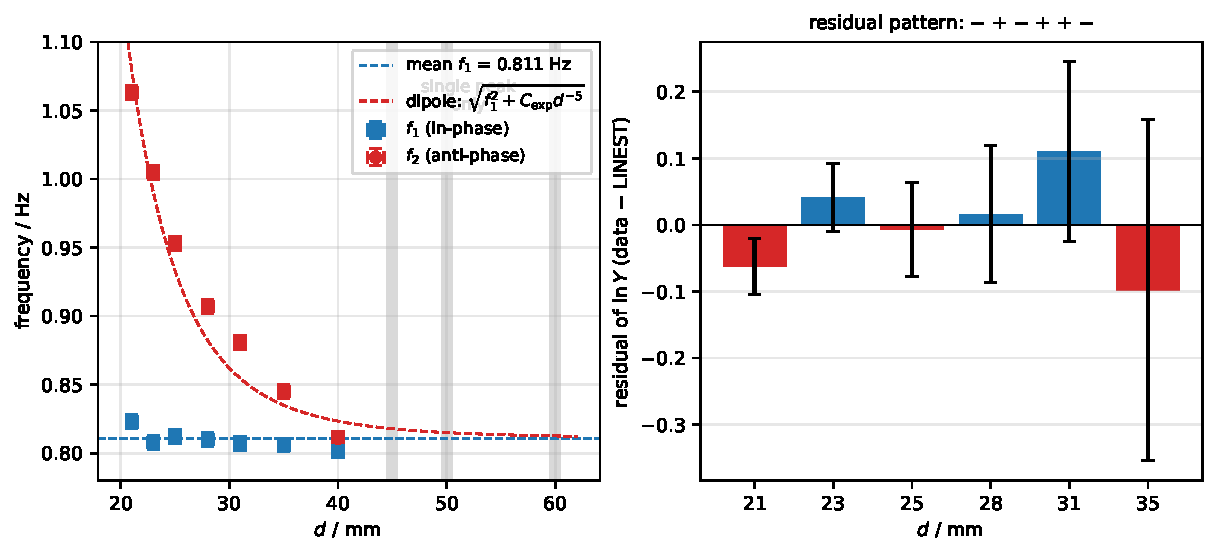
\includegraphics[width=\textwidth]{G3_f_vs_d}
\caption{Graph 3. Left: $f_1$ and $f_2$ against $d$; the dashed red curve is the dipole prediction $\sqrt{f_1^2+C_{\rm exp}d^{-5}}$ with $C_{\rm exp}$ from Graph 2, and the grey bands mark the separations at which only one peak was found. Right: residuals of $\ln\Y$ from the unweighted line of Graph 1.}
\label{fig:G3}
\end{figure}

\subsection{Graph 4: average frequency and beat frequency}

The research question also asks for the two derived quantities $f_{\rm avg}=(f_1+f_2)/2$ and $f_{\rm beat}=f_2-f_1$. Their uncertainties follow from those of $f_1$ and $f_2$ by adding in quadrature: $\Delta f_{\rm avg}=\Delta f/\sqrt2=0.004\un{Hz}$ and $\Delta f_{\rm beat}=\sqrt2\,\Delta f=0.007\un{Hz}$. Figure~\ref{fig:G4} shows both against $d$, together with the predictions of equation~\eqref{eq:favg_fbeat} evaluated with the mean $f_1$ and the $C_{\rm exp}$ of Graph~2.

The average frequency behaves as predicted: it is essentially constant at $f_1$ for $d\gtrsim30\un{mm}$ and rises to $\nfavgSmall\un{Hz}$ at $21\un{mm}$ (prediction $\nfavgPredSmall\un{Hz}$), a rise of $16\,\%$ that is entirely due to $f_2$. The beat frequency falls from $\nfbeatSmall\un{Hz}$ at $21\un{mm}$ (beat period $\nTbeatSmall\un{s}$) to $\nfbeatLarge\un{Hz}$ at $40\un{mm}$ (beat period $\nTbeatLarge\un{s}$, i.e.\ longer than the $30\un{s}$ record, which is why the two peaks were not resolved there). On the log--log axes of the right-hand panel the six resolved points lie close to a straight line of gradient $\ngradBeat\pm\ngradBeatErr$, and at $45$--$60\un{mm}$ only upper limits can be given ($f_{\rm beat}<1/T=33\un{mHz}$, the bin width). The dipole prediction would put the beat period at $60\un{mm}$ near $\nTbeatPredSixty\un{min}$ ($f_{\rm beat}\approx\nfbeatPredSixty\un{mHz}$), far below what a $30\un{s}$ record can resolve. Because $f_{\rm beat}=\Y/(2f_{\rm avg})$ and $f_{\rm avg}$ changes by only $16\,\%$, the beat-frequency graph carries the same information as Graph~1, and its gradient is shallower than $-5$ by the same amount; the exponent problem is therefore analysed once, on $\Y$, in the sections that follow.

\begin{figure}[htbp]
\centering
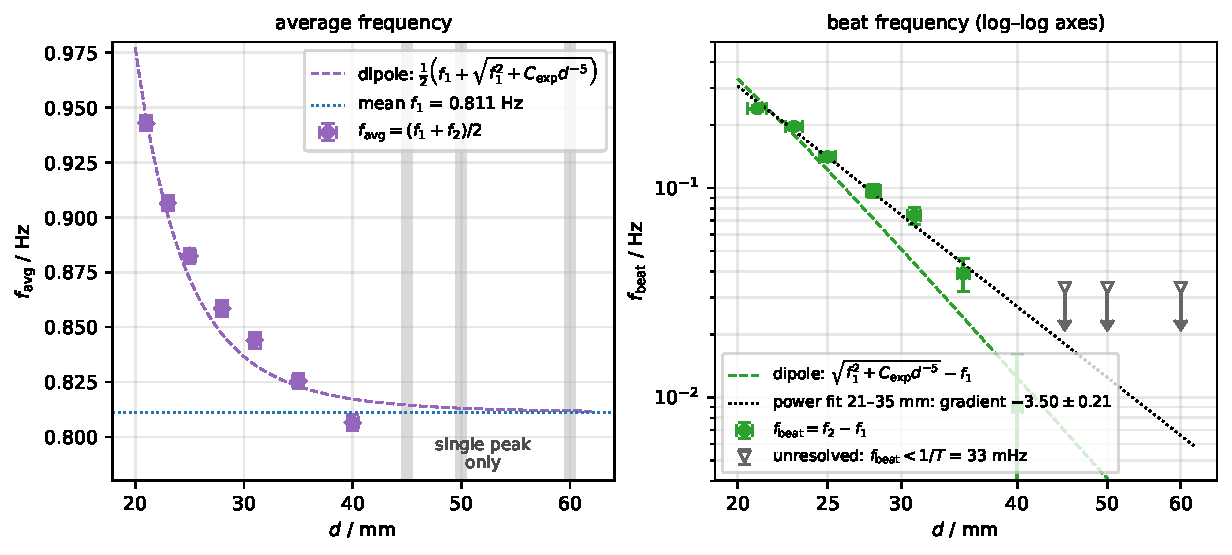
\includegraphics[width=\textwidth]{G4_favg_fbeat}
\caption{Graph 4. Left: average frequency $f_{\rm avg}$ against $d$ with the dipole prediction of equation~\eqref{eq:favg_fbeat}. Right: beat frequency $f_{\rm beat}=f_2-f_1$ on log--log axes with the dipole prediction (dashed), a free power-law fit to the six resolved points (dotted) and upper limits at the three separations where only one peak was found.}
\label{fig:G4}
\end{figure}

\subsection{Comparison with the theoretical values}

\begin{table}[htbp]
\centering\footnotesize
\caption{Measured against predicted values.}
\label{tab:compare}
\setlength{\tabcolsep}{4pt}
\begin{tabular}{@{}p{6.4cm}p{3.1cm}p{2.9cm}p{2.6cm}@{}}
\toprule
Quantity & Predicted & Measured & Difference \\
\midrule
Exponent $n$ in $\Y\propto d^{-n}$ (Graph 1, unweighted) & $5$ & $3.75\pm0.19$ & $-25\,\%$ ($6.4\sigma$)\\
Exponent $n$ (Graph 1, weighted) & $5$ & $3.48\pm0.24$ & $-30\,\%$ ($6.3\sigma$)\\
Exponent $n$ (non-linear fit to $\Y$, Section~\ref{sec:nonlinfit}) & $5$ & $\nnFree\pm\nnFreeErr$ & $-30\,\%$\\
$C$ / $\mathrm{m^5\,s^{-2}}$ (Graph 2, through origin) & $3\muz\mum^2/(\pi^3 m)$ $=\TBM{\ldots}$ & $(2.08\pm0.15)\times10^{-9}$ & \TBM{\ldots}\\
$\mum^2/m$ / $\mathrm{A^2m^4kg^{-1}}$ implied by $C_{\rm exp}$ & \TBM{from $\mum$, $m$} & $\nmmFromC$ & \TBM{\ldots}\\
$f_1$ against $d$ & constant & falls by $2.6\,\%$ over 21--40 mm & $\approx4\sigma$\\
Exponent of $f_{\rm beat}$ against $d$ (Graph 4, 21--35 mm) & $\approx-5$ (weak coupling) & $\ngradBeat\pm\ngradBeatErr$ & $-30\,\%$\\
\bottomrule
\end{tabular}
\end{table}

The exponent is the central result. It is measured with a precision of about $5\,\%$ and disagrees with the dipole prediction by $25$--$30\,\%$. Random error cannot account for a discrepancy of six standard errors, so a systematic explanation must be found; this is the task of the next two sections.

\section{Discussion of the preliminary results}\label{sec:discussion}

The qualitative predictions of Section~2 are confirmed. The coupling term $\Y=f_2^2-f_1^2$ falls steeply with separation, by a factor of $7$ between $21$ and $35\un{mm}$; $f_2$ approaches $f_1$; the beats slow down until, beyond $40\un{mm}$, the two frequencies can no longer be separated in a $30\un{s}$ record; and the dependence is well described by a power law, as the straightness of Graph~1 shows ($R^2=0.989$). The magnetic force does act as a tunable coupling spring, and the coupling can be switched from strong ($2\gamma/k\approx0.7$) to negligible by moving the clamps by a few centimetres.

Quantitatively, however, the data disagree with the point-dipole model in four related ways:
\begin{enumerate}
\item the exponent is $\ngradSix\pm\ngradSixErr$ rather than $-5$;
\item $f_1$ is not constant but rises by $2.6\,\%$ as the magnets approach;
\item the through-origin line of Graph~2 does not fit, a free intercept of $0.06\un{Hz^2}$ being required;
\item the residuals of Graph~1 hint at a concave-down curvature.
\end{enumerate}

It is tempting to conclude that the force between the magnets simply falls as $d^{-3.75}$ rather than $d^{-5}$. But that would contradict a very well established law, and there are several ways in which the \emph{measurement} and the \emph{model} could each produce exactly this kind of deviation. They fall into two families.

\paragraph{Measurement effects.} The frequencies are read from spectra of $30\un{s}$ records. Section~\ref{sec:fftbackground} showed that two peaks closer than $1$--$2$ bins ($33$--$67\un{mHz}$) pull on each other or merge; at $31$ and $35\un{mm}$ the separation is $2.2$ and $1.2$ bins, so the frequencies at the large-$d$ end of the graph, precisely the points that determine the gradient, are the least trustworthy. The release amplitude of $10\un{mm}$ is almost half the smallest separation, so the assumption of small displacements is questionable at the small-$d$ end.

\paragraph{Model effects.} The magnets are not points ($d/D$ of order $2$--$6$); the two springs are not exactly identical; the cantilever tip tilts as it bends; there is damping. Each of these was listed as an assumption in Section~\ref{sec:remarks}.

The strategy of the rest of the essay is to take each effect in turn, work out the \emph{sign} of the error it produces in the gradient of Graph~1, estimate its \emph{size} with the measured numbers, and identify a \emph{remedy}. An effect can only explain the discrepancy if it makes the gradient \emph{shallower} (less negative) than $-5$ by an amount of order $1$; effects that make it steeper, however large, cannot be the culprit and must in fact be corrected for \emph{before} the shallowing effects can be assessed. Section~\ref{sec:evaluation} does this analysis; Sections~\ref{sec:further}--\ref{sec:simulation} then apply the remedies.

\section{Evaluation}\label{sec:evaluation}

Each sub-section below treats one source of error and ends with its \textbf{sign} (the direction in which it moves the gradient of Graph~1), its \textbf{size} for the conditions of this experiment, and its \textbf{remedy}. Table~\ref{tab:errsummary} at the end collects the results.

\subsection{FFT resolution, leakage and peak pulling (measurement; assumption g)}\label{sec:fftres}

\paragraph{Resolvability.} Table~\ref{tab:resolution} lists, for each separation, the measured peak spacing $f_2-f_1$, the number of bins it corresponds to at $T=30\un{s}$, and the minimum record length for the two peaks to be one bin apart (rectangular window) or two bins apart (Hann). At $21$--$28\un{mm}$ the peaks are $3$--$7$ bins apart and well resolved. At $31\un{mm}$ they are $2.2$ bins apart, at $35\un{mm}$ only $1.2$ bins, and at $40\un{mm}$ $0.3$ bins: the last is not resolvable in principle with a $30\un{s}$ record, and the two values listed for it in Table~\ref{tab:rawfreq} are the positions of a merged peak and its shoulder, not two frequencies. Beyond $40\un{mm}$ a record of $2$--$10$ minutes would be needed, longer than the oscillation lasts.

\paragraph{Peak pulling.} To find out how much the overlapping lobes displace the peaks that \emph{are} resolved, synthetic records were generated with exactly the measured frequencies of each row, the measured decay time, the actual frame rate and record length, and a realistic amount of tracking noise, and then analysed with exactly the same procedure as the data (Appendix~\ref{app:code}, Part~A). The last six columns of Table~\ref{tab:resolution} give the error (recovered minus true) for each frequency. With the rectangular window at $T=30\un{s}$ the peaks are pushed \emph{apart} by $1$--$4\un{mHz}$ each, i.e.\ $f_2-f_1$ is overestimated by $2$--$8\un{mHz}$, rising with $d$; with the Hann window the errors are smaller at small $d$ but at $35\un{mm}$ the two four-bin-wide lobes overlap so much that the peaks are pulled by $13\un{mHz}$; at $40\un{mm}$ the Hann spectrum shows a single peak. With $T=90\un{s}$ all errors fall below $1$--$2\un{mHz}$ up to $40\un{mm}$. Figure~\ref{fig:resolution} shows the corresponding spectra.

\begin{table}[htbp]
\centering\footnotesize
\caption{Resolvability of the two peaks, and the peak-position errors (recovered $-$ true, in mHz) obtained by analysing synthetic two-tone records with the frequencies of each row ($\tau=25\un{s}$, $240\un{fps}$, $0.1\un{mm}$ rms tracking noise) with the same procedure as the data. `--' = only one peak found.}
\label{tab:resolution}
\setlength{\tabcolsep}{4pt}
\begin{tabular}{@{}c c c cc cc cc cc@{}}
\toprule
$d$ & $f_2-f_1$ & bins & \multicolumn{2}{c}{$T_{\min}$ / s} & \multicolumn{2}{c}{$T=30$ s, rect} & \multicolumn{2}{c}{$T=30$ s, Hann} & \multicolumn{2}{c}{$T=90$ s, rect}\\
/ mm & / Hz & at 30 s & rect & Hann & $\delta f_1$ & $\delta f_2$ & $\delta f_1$ & $\delta f_2$ & $\delta f_1$ & $\delta f_2$\\
\midrule
\tabinput{tables/tab_resolution}
\bottomrule
\end{tabular}
\end{table}

\begin{figure}[htbp]
\centering
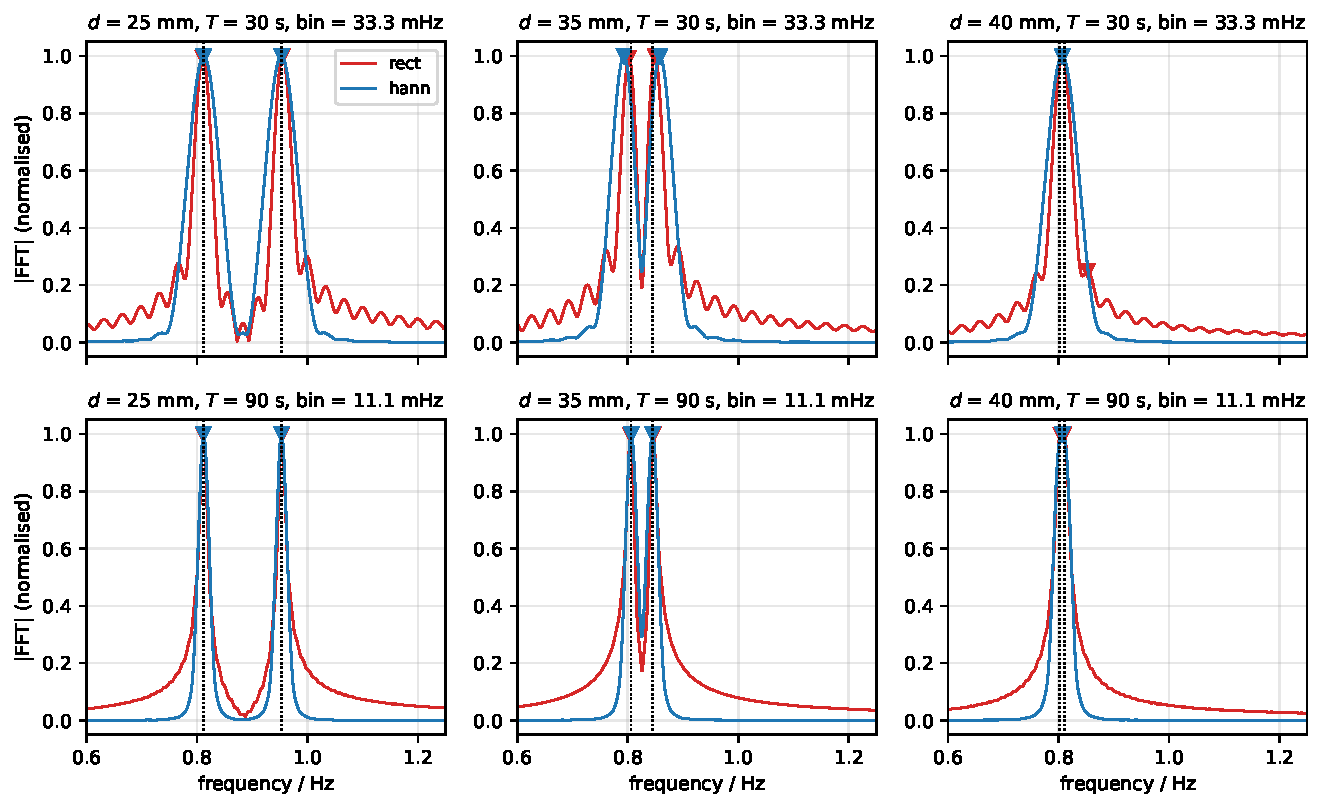
\includegraphics[width=\textwidth]{F_resolution}
\caption{Synthetic two-tone spectra with the measured frequencies at $25$, $35$ and $40\un{mm}$ (dotted lines) for $T=30\un{s}$ (top, as in the experiment) and $T=90\un{s}$ (bottom), rectangular (red) and Hann (blue) windows; triangles mark the detected peaks. At $35\un{mm}$ the $30\un{s}$ Hann spectrum barely resolves the peaks and pulls them; at $40\un{mm}$ neither window resolves them.}
\label{fig:resolution}
\end{figure}

\paragraph{Effect on the gradient.} A positive error in $f_2-f_1$ that grows with $d$ inflates $\Y$ most at the large-$d$ end and therefore makes the gradient of Graph~1 \emph{shallower}. The errors look small in absolute terms, but at $35\un{mm}$ an extra $8\un{mHz}$ on a spacing of $39\un{mHz}$ is a $20\,\%$ overestimate of $f_2-f_1$ and hence a $26\,\%$ overestimate of $\Y$, against $1\,\%$ at $21\un{mm}$. Subtracting the Table~\ref{tab:resolution} errors from the measured frequencies moves the measured gradient from $\ngradSix$ to $-4.14$; equivalently, in the synthetic test of Section~\ref{sec:simulation}, a system that obeys the dipole law exactly appears to have a gradient of $\ngradPullOnly$ when analysed with a $30\un{s}$ record and a rectangular window. The effect therefore has the right sign and accounts for roughly one third of the discrepancy, but not all of it. Its second consequence is the loss of every point beyond $35\un{mm}$, which halves the usable range of $\ln d$ and makes the gradient hostage to the two least reliable points. A third consequence concerns $f_1$: the pulling pushes $f_1$ \emph{down} by an amount that grows with $d$ (Table~\ref{tab:resolution}), so part of the observed fall of $f_1$ with $d$ ($21\un{mHz}$ between $21$ and $40\un{mm}$) is an analysis artefact; the simulation of the original procedure reproduces about $\noldFoneDrift\un{mHz}$ of it.

\paragraph{Damping linewidth.} With $\tau\approx25\un{s}$ the intrinsic linewidth $\nlwAmp\un{Hz}$ (Section~\ref{sec:fftbackground}) is already comparable to $f_2-f_1$ at $35\un{mm}$ and larger than it at $40\un{mm}$. Lengthening the record therefore helps only up to $T\sim2\tau$; beyond $\sim40\un{mm}$ no spectral analysis of a single coordinate can separate the modes, however long the record. Escaping this limit requires either a different coordinate (Section~\ref{sec:further}, normal coordinates) or a different estimator (time-domain fitting).

\paragraph{Sign, size, remedy.} \textbf{Sign:} shallower. \textbf{Size:} $+2$--$8\un{mHz}$ in $f_2-f_1$ at $T=30\un{s}$; gradient $-5.0\to\ngradPullOnly$; all points beyond $35\un{mm}$ lost. \textbf{Remedy:} $T\geq90\un{s}$; track both magnets and transform the normal coordinates; fit two damped sinusoids in the time domain (Section~\ref{sec:further}).

\subsection{Amplitude non-linearity of the magnetic force (model; assumption b)}\label{sec:nonlinear}

Equation~\eqref{eq:eom} kept only the first-order term of $F(d+u)$. The repulsive force $F\propto r^{-4}$ is convex: it rises more steeply when the magnets approach than it falls when they recede. Over a full anti-phase swing of amplitude $a$ the average restoring force is therefore \emph{larger} than the linear term $\gamma u$, so the effective stiffness of the anti-phase mode increases with amplitude. This is a \emph{hardening} non-linearity, and its consequence is that a finite-amplitude measurement \emph{over}estimates $f_2$.

Quantitatively, expanding $F(d-\xi)-F(d)$ to third order in the anti-phase coordinate $\xi=x_1-x_2$ (Appendix~\ref{app:nonlinear}) gives the equation of motion
\begin{equation}
\ddot\xi+\omega_2^2\xi+\alpha\xi^2+\beta\xi^3=0,\qquad
\alpha=\frac52\,\frac{g\,\omega_2^2}{d},\quad
\beta=\frac{5\,g\,\omega_2^2}{d^2},\quad
g\equiv\frac{f_2^2-f_1^2}{f_2^2},
\label{eq:duffing}
\end{equation}
where $g$ is the fraction of the anti-phase stiffness that is magnetic. The standard perturbation result for the frequency of such an oscillator at amplitude $a$ \cite{landau} is
\begin{equation}
\frac{\Delta\omega}{\omega_2}=\left(\frac{3\beta}{8\omega_2^2}-\frac{5\alpha^2}{12\omega_2^4}\right)a^2
=\left(\frac{a}{d}\right)^2\left(\frac{15g}{8}-\frac{125g^2}{48}\right)>0 .
\label{eq:LL}
\end{equation}
For the release used here the anti-phase amplitude is close to the release displacement, $a=\xi_0\approx A=10\un{mm}$ (equation~\eqref{eq:solution}; the hold-and-release correction of equation~\eqref{eq:heights} reduces it by about $20\,\%$, which only weakens the shifts estimated below). At $d=21\un{mm}$, $g=0.40$ and $a/d=0.48$, giving $\Delta\omega/\omega_2=+7\,\%$; at $35\un{mm}$, $g=0.09$, $a/d=0.29$ and the shift is $+0.9\,\%$. Because $a/d$ is far from small at $21\un{mm}$ the perturbation series is not reliable there, so the full non-linear equations of motion were also integrated numerically (Section~\ref{sec:simulation}); the results, Table~\ref{tab:amplitude} and Figure~\ref{fig:amplitude}, confirm the sign and show that the true shift at $21\un{mm}$ is $+\nshiftTwentyOneAten\,\%$, somewhat larger than the perturbation estimate. The frequency shift measured in a real record is smaller than these initial values because the amplitude decays during the $30\un{s}$ record and the FFT peak represents an average; but the average is still positive.

\begin{table}[htbp]
\centering\small
\caption{Percentage increase of $f_2$ relative to its small-amplitude value, from numerical integration of the full dipole-force equations with the parameters of this experiment; last column: perturbation formula~\eqref{eq:LL} for $A=10\un{mm}$.}
\label{tab:amplitude}
\begin{tabular}{@{}c c cccccc c@{}}
\toprule
$d$ / mm & $f_2(A\to0)$ / Hz & $A=1$ & 2 & 3 & 5 & 7 & 10 mm & eq.~\eqref{eq:LL}, 10 mm\\
\midrule
\tabinput{tables/tab_amplitude}
\bottomrule
\end{tabular}
\end{table}

\begin{figure}[htbp]
\centering
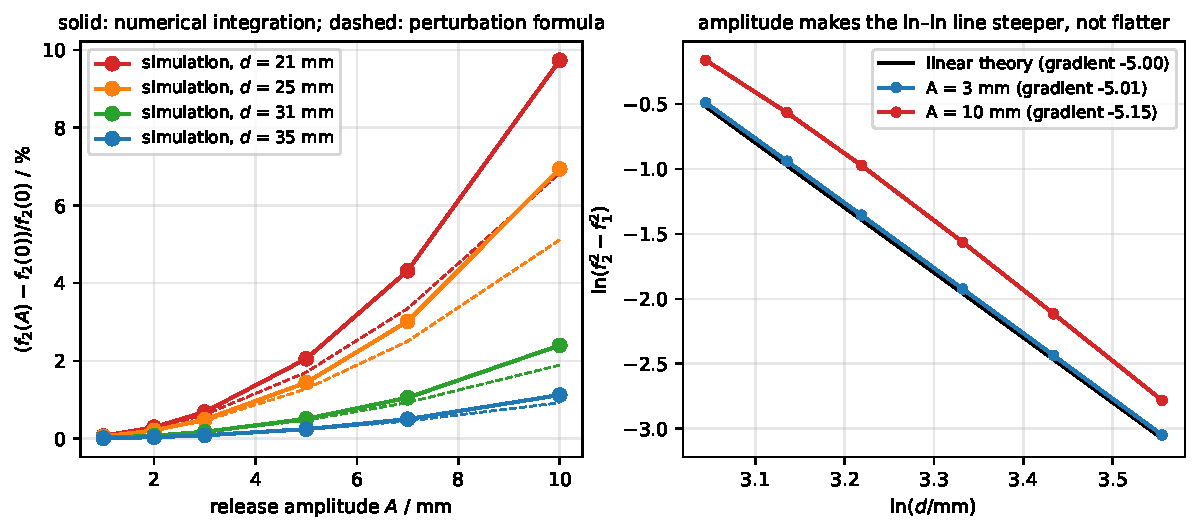
\includegraphics[width=\textwidth]{F_amplitude}
\caption{Left: amplitude dependence of $f_2$ from the numerical integration (solid) and the perturbation formula (dashed). Right: the effect on Graph 1. Because the shift is largest at small $d$, a finite release amplitude makes the ln--ln line \emph{steeper}, not shallower: gradient $\ngradAthree$ for $A=3\un{mm}$, $\ngradAten$ for $A=10\un{mm}$.}
\label{fig:amplitude}
\end{figure}

\paragraph{Effect on the gradient.} The overestimate of $f_2$ is largest at the \emph{small}-$d$ end, where $\Y$ is largest. It therefore lifts the left-hand end of Graph~1 and makes the gradient \emph{steeper}: $-5.00\to\ngradAten$ for $A=10\un{mm}$ in the simulation. This is the opposite of what is observed. The amplitude non-linearity therefore cannot explain the measured $-3.75$; on the contrary, the measured gradient, once corrected for it, would be even shallower, so the shallowing effects discussed next must be somewhat larger than the raw discrepancy suggests.

\paragraph{Tilt of the magnets (assumption f).} A related consequence of finite amplitude is that the tip of a cantilever does not translate; it rotates by the tip slope $\theta\simeq3A/(2L)$ (Appendix~\ref{app:cantilever}), which for $A=10\un{mm}$ and $L=\TBM{150}\un{mm}$ is $\ntiltRad\un{rad}=\ntiltDeg^\circ$. The interaction energy of two dipoles at angles $\alpha_1,\alpha_2$ to their common axis is proportional to $3\cos\alpha_1\cos\alpha_2-\cos(\alpha_1-\alpha_2)$ (Appendix~\ref{app:dipole}); for the equal-and-opposite tilts of the anti-phase motion the factor $2$ of the coaxial case becomes $2-\theta^2$, a weakening of the magnetic stiffness by $\theta^2/2\approx0.5\,\%$ at the extreme of the swing (and $2-3\theta^2$, i.e.\ $1.5\,\%$, for the equal tilts of the in-phase motion, where the separation does not change and the effect is irrelevant). Averaged over a cycle and decaying with the amplitude, the effect on $\Y$ is a few tenths of a per cent and independent of $d$ to first order, so it does not affect the gradient. \textbf{Sign:} steeper (amplitude), negligible (tilt). \textbf{Size:} $f_2$ $+\nshiftTwentyOneAten\,\%$ at $21\un{mm}$, $+\nshiftThirtyFiveAten\,\%$ at $35\un{mm}$ for $A=10\un{mm}$; below $0.7\,\%$ everywhere for $A=3\un{mm}$. \textbf{Remedy:} release with $A\leq3\un{mm}$; analyse late (small-amplitude) segments of each record; extrapolate $f_2$ to zero amplitude (Section~\ref{sec:furtherdata}).

\subsection{Finite size of the magnets (model; assumption a)}\label{sec:finite}

The point-dipole force law is the leading term of an expansion in $D/d$. A real cylindrical magnet can be modelled exactly (for uniform magnetisation) by two uniformly ``charged'' discs of opposite sign, one on each flat face, whose surface pole density is $\pm B_r/\muz$ \cite{griffiths}; the force between two magnets is then the sum of the Coulomb-like forces between the four discs (Appendix~\ref{app:finite}). Two effects follow. First, the nearest faces of the two magnets are closer than the centres, and the farthest faces are farther away, so the force at a given $d$ differs from the dipole value. Second, and decisively, the charge on each face is spread over a disc of radius $D/2$: at separations comparable to $D$ much of the disc-to-disc force acts obliquely and partly cancels, so the axial force is \emph{weaker} than the point-dipole formula predicts, and the shortfall grows as $d$ decreases (Figure~\ref{fig:finite}, left).

A force that is depressed below $d^{-4}$ at small $d$ has a magnetic stiffness $\gamma=-\dd F/\dd d$ that falls \emph{more slowly} than $d^{-5}$ over the measured range. The apparent gradient of $\ln\gamma$ against $\ln d$ over $21$--$35\un{mm}$, computed with this model, is given in Table~\ref{tab:finite} and Figure~\ref{fig:finite} (right) for several magnet sizes: $\nfsGradSix$ for a $6\un{mm}$ magnet, $\nfsGradTen$ for $10\un{mm}$, $\nfsGradFifteen$ for $15\un{mm}$ and $\nfsGradTwenty$ for $20\un{mm}$, nearly independent of the thickness $t$. The finite size of the magnets is therefore the one effect examined so far that has both the right \emph{sign} and a plausible \emph{size}: a magnet of diameter $\approx\TBM{D}\un{mm}$ \TBM{compare with the actual magnet} would account for essentially all of the discrepancy. The model also predicts a concave-down curvature of the ln--ln plot (the local gradient steepens towards $-5$ as $d$ grows), which is the pattern hinted at by the residuals in Figure~\ref{fig:G3}.

\begin{table}[htbp]
\centering\small
\caption{Apparent gradient of $\ln\gamma$ against $\ln d$ over $21$--$35\un{mm}$ for cylindrical magnets of diameter $D$ and thickness $t$, from the charged-disc model (Appendix~\ref{app:finite}). The point-dipole value is $-5$.}
\label{tab:finite}
\begin{tabular}{@{}ccc@{}}
\toprule
$D$ / mm & $t$ / mm & apparent gradient\\
\midrule
\tabinput{tables/tab_finite}
\bottomrule
\end{tabular}
\end{table}

\begin{figure}[htbp]
\centering
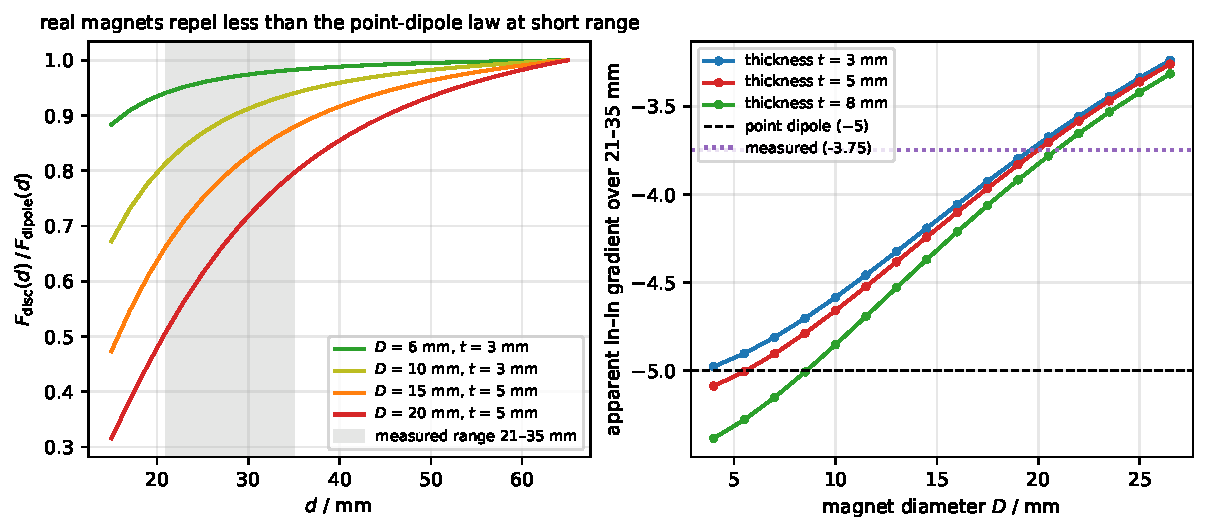
\includegraphics[width=\textwidth]{F_finite_size}
\caption{Finite-size effect. Left: ratio of the exact force between two uniformly magnetised cylinders (charged-disc model) to the point-dipole force, normalised at $65\un{mm}$; the grey band is the measured range. Right: apparent ln--ln gradient of the magnetic stiffness over $21$--$35\un{mm}$ against magnet diameter. A $20\un{mm}$ magnet reproduces the measured gradient exactly; the actual magnet size is \TBM{$D$}.}
\label{fig:finite}
\end{figure}

\paragraph{Sign, size, remedy.} \textbf{Sign:} shallower. \textbf{Size:} gradient $-5\to\nfsGradSix$ ($D=6\un{mm}$) \ldots $\nfsGradTwenty$ ($D=20\un{mm}$) over $21$--$35\un{mm}$. \textbf{Remedy:} replace the point-dipole force by the finite-size force in the model (Section~\ref{sec:nonlinfit}), or measure at $d\gtrsim4D$ where the dipole law is accurate to a few per cent, which collides with the resolution problem of Section~\ref{sec:fftres} and forces the improvements of Section~\ref{sec:further}.

\subsection{Non-identical springs (model; assumption c)}\label{sec:detuned}

If the two springs have different uncoupled angular frequencies $\omega_a\neq\omega_b$ (because of small differences in $L$, $h$, clamping or magnet mass), the in-phase mode no longer leaves the coupling untouched. Solving the coupled equations with $k_a/m_a=\omega_a^2$, $k_b/m_b=\omega_b^2$ and equal masses (Appendix~\ref{app:detuned}) gives
\begin{equation}
\omega_{1,2}^2=\bar\omega^2+\kappa\mp\sqrt{\Delta^2+\kappa^2},\qquad
\kappa=\frac{\gamma}{m},\quad
\Delta=\frac{\omega_b^2-\omega_a^2}{2},\quad
\bar\omega^2=\frac{\omega_a^2+\omega_b^2}{2},
\label{eq:detuned}
\end{equation}
which reduces to \eqref{eq:modes} when $\Delta=0$. Two limits explain the observations. When the coupling is weak ($\kappa\ll\Delta$, large $d$), $\omega_1\to\omega_a$ and $\omega_2\to\omega_b$: the ``modes'' are just the two springs oscillating separately at their own frequencies, and $f_2^2-f_1^2$ saturates at $|f_b^2-f_a^2|$ instead of tending to zero. When the coupling is strong ($\kappa\gg\Delta$), $\omega_1^2\to\bar\omega^2$ from below, so \emph{$f_1$ rises as the magnets approach} and levels off at $\bar f$, while $\omega_2^2\to\bar\omega^2+2\kappa$ grows without bound. Squaring and subtracting the two roots of \eqref{eq:detuned} gives the modified test relation
\begin{equation}
\Y^2=\big(f_b^2-f_a^2\big)^2+\big(Cd^{-5}\big)^2 ,
\label{eq:detunedY}
\end{equation}
so a ln--ln plot of $\Y$ is a straight line of gradient $-5$ only where $Cd^{-5}\gg|f_b^2-f_a^2|$, and flattens towards a horizontal asymptote at large $d$.

Both predicted signatures are present in the data: $f_1$ rises from $0.802$ to $0.823\un{Hz}$ as $d$ falls, and the large-$d$ end of Graph~1 is flatter than the small-$d$ end. Fitting \eqref{eq:detuned} to all twelve resolved frequencies with $f_a$, $f_b$ and $C$ free (Figure~\ref{fig:detuned}) gives $f_a=\nfaFit\pm\nfaFitErr\un{Hz}$ and $f_b=\nfbFit\pm\nfbFitErr\un{Hz}$, a detuning of $7\,\%$; the fitted curve reproduces the drift of $f_1$ ($\ndetFoneLarge\to\ndetFoneSmall\un{Hz}$ against the observed $0.802\to0.823\un{Hz}$) and halves the residual sum of squares compared with the identical-spring dipole model ($\chi^2$ from $\nchiIdentical$ to $\nchiDetuned$ for the same number of points). The fit is not perfect, and a $7\,\%$ detuning is larger than expected from the construction tolerances, so this explanation must be checked directly by measuring $f_a$ and $f_b$ with each spring alone (Section~\ref{sec:further}); but it is the only mechanism identified that explains the drift of $f_1$. A second, independent check is already available in the beat records: for identical springs the ratio of the two peak heights must be the same in the spectra of spring~1 and spring~2 (Section~\ref{sec:modes}), whereas for detuned springs the in-phase mode shape tilts from $(1,1)$ to $(a_1,b_1)$ and the ratios differ by the factor $(a_1/b_1)^2$, with $a_1/b_1-b_1/a_1=2\Delta/\kappa$. In the record of Figure~\ref{fig:beats_example} the two ratios differ by about $10\,\%$, which corresponds to $|f_b-f_a|\approx0.01\un{Hz}$ (about $1\,\%$, spring~2 the stiffer)---much smaller than the $0.056\un{Hz}$ of the fit. \TBM{Recompute from the final records with \texttt{plot\_beats.py}, which prints $r_1$, $r_2$ and the implied $f_b-f_a$.} Taken together, the peak-height test suggests that detuning is real but too small to be the main cause of the shallow gradient.

\begin{figure}[htbp]
\centering
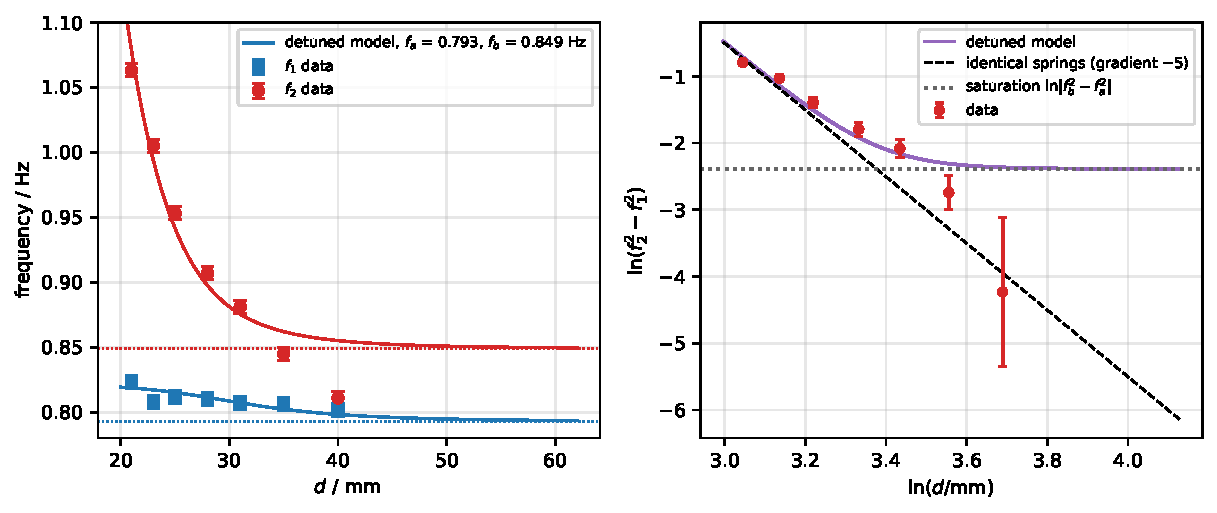
\includegraphics[width=\textwidth]{F_detuned}
\caption{Non-identical springs. Left: $f_1$, $f_2$ data with the detuned model \eqref{eq:detuned} fitted ($f_a=\nfaFit$, $f_b=\nfbFit\un{Hz}$); the dotted lines are the fitted uncoupled frequencies. Right: the same model in the ln--ln plane: it follows the dipole line at small $d$ and bends towards the saturation value $\ln|f_b^2-f_a^2|$ at large $d$.}
\label{fig:detuned}
\end{figure}

\paragraph{Sign, size, remedy.} \textbf{Sign:} shallower, increasingly so at large $d$; also produces the observed rise of $f_1$. \textbf{Size:} with $f_b-f_a=0.056\un{Hz}$, $\Y$ saturates at $\nYsatDetuned\un{Hz^2}$, which is already comparable to the measured $\Y$ at $35\un{mm}$. \textbf{Remedy:} measure $f_a$, $f_b$ directly and fit equation~\eqref{eq:detunedY} with them fixed; match the springs (trim $L$) so that $|f_b-f_a|<0.005\un{Hz}$.

\subsection{Damping and other minor effects (assumptions d, e)}

\paragraph{Damping.} Light damping lowers the frequency of an oscillator by a fraction $\tfrac12(1/2\omega\tau)^2$; with $\tau=25\un{s}$ and $\omega\approx5\un{s^{-1}}$ this is $10^{-5}$, utterly negligible. Damping matters only through its linewidth (Section~\ref{sec:fftres}). Eddy-current damping of the magnets by the copper strip is part of the measured $\tau$.

\paragraph{Lumped mass.} The numerical comparison of the lumped model with the continuous beam (Appendix~\ref{app:cantilever}) gives an error in $\Y$ of $0.4\,\%$ for $M/\mu L=0.8$ and $1\,\%$ for $0.4$; the ratio here is \TBM{$M/\mu L=\ldots$}. Because the error is the same at every $d$ it changes $C$ slightly but not the gradient.

\paragraph{Distance.} $\Delta d=0.5\un{mm}$ is $2.4\,\%$ of $21\un{mm}$ and enters $\Y$ five-fold, i.e.\ $12\,\%$; it is the dominant contribution to the horizontal error bars at small $d$ and a strong argument for reading $d$ from a calibrated video frame rather than with a rule. A \emph{systematic} error in $d$, such as measuring the gap $g$ instead of $g+t$, or setting the clamp separation before the magnets push the springs apart, would offset every $d$ by roughly the same amount. Table~\ref{tab:deflection} shows what the second mistake would have done: the outward deflection $2\delta$ calculated from the data ranges from $3.7\un{mm}$ at $21\un{mm}$ to $0.2\un{mm}$ at $40\un{mm}$, and plotting $\Y$ against the clamp separation $d-2\delta$ instead of the true $d$ would change the gradient from $\ngradSix$ to $\ngradSet$. Conversely, the fact that $d$ \emph{was} read at equilibrium means that this particular error is absent, but the size of the effect shows how sensitive the exponent is to the definition of $d$.

\begin{table}[htbp]
\centering\small
\caption{Static outward deflection $\delta$ of each spring, calculated from the measured frequencies ($\delta=\pi^2\Y d/2\omega_1^2$, Section~\ref{sec:remarks}), and the clamp separation that would have produced each $d$.}
\label{tab:deflection}
\begin{tabular}{@{}ccccc@{}}
\toprule
$d$ / mm & $\Y$ / Hz$^2$ & $\delta$ / mm & $d+2\delta$ / mm & $2\delta/d$ / \%\\
\midrule
\tabinput{tables/tab_deflection}
\bottomrule
\end{tabular}
\end{table}

\subsection{Random errors}

The random uncertainty of $\pm5\un{mHz}$ assigned to each frequency comes from the half-range of the three trials at each $d$, which reflects tracking noise, frame-timing jitter and the repeatability of the release and of $d$. With zero-padding and parabolic interpolation the bin-centring error is removed; tracking noise of $0.1\un{mm}$ rms on a $10\un{mm}$ oscillation sampled $7200$ times contributes well under $1\un{mHz}$. The random errors are therefore small compared with the systematic ones identified above, which is consistent with the smallness of the residual scatter about the (wrong) straight line of Graph~1.

\subsection{Summary of systematic effects}

\begin{table}[htbp]
\centering\footnotesize
\caption{Systematic effects, their direction on the gradient of Graph 1, their size under the conditions of the original measurements, and the remedy applied in Sections~\ref{sec:further}--\ref{sec:simulation}.}
\label{tab:errsummary}
\setlength{\tabcolsep}{4pt}
\renewcommand{\arraystretch}{1.15}
\begin{tabular}{@{}>{\raggedright\arraybackslash}p{2.6cm}>{\raggedright\arraybackslash}p{1.9cm}>{\raggedright\arraybackslash}p{3.0cm}>{\raggedright\arraybackslash}p{4.0cm}>{\raggedright\arraybackslash}p{3.5cm}@{}}
\toprule
Effect & Type & Sign on gradient & Size (this experiment) & Remedy\\
\midrule
FFT resolution, peak pulling, linewidth & measurement (g) & shallower; large-$d$ points lost & $+2$ to $+8\un{mHz}$ in $f_2-f_1$ at $T=30\un{s}$; gradient $-5.0\to\ngradPullOnly$; nothing beyond 35\,mm & $T\geq90\un{s}$; normal-coordinate FFT; two-tone time-domain fit\\[2pt]
Amplitude non-linearity (hardening) & model (b) & \emph{steeper} & $f_2$ $+\nshiftTwentyOneAten\,\%$ (21\,mm), $+\nshiftThirtyFiveAten\,\%$ (35\,mm) at $A=10\un{mm}$; gradient $-5.00\to\ngradAten$ & $A\leq3\un{mm}$; segment analysis; extrapolation to $a\to0$\\[2pt]
Finite magnet size & model (a) & shallower & gradient $-5\to\nfsGradTen$ ($D=10\un{mm}$), $\nfsGradTwenty$ ($D=20\un{mm}$) & finite-size force in the fit; $d\gtrsim4D$\\[2pt]
Non-identical springs & model (c) & shallower at large $d$; $f_1$ rises at small $d$ & $f_b-f_a\approx0.06\un{Hz}$ (fit); $\Y$ saturates at $\nYsatDetuned\un{Hz^2}$ & measure $f_a$, $f_b$; fit eq.~\eqref{eq:detunedY}; match springs\\[2pt]
Tilt of magnets & model (f) & none (same at all $d$) & $<1\,\%$ of $\Y$ & $A\leq3\un{mm}$\\[2pt]
Damping & model (e) & none & $10^{-5}$ shift; linewidth $\nlwAmp\un{Hz}$ & --\\[2pt]
Lumped mass & model (d) & none & $<1\,\%$ of $C$ & --\\[2pt]
Distance $d$ & random / systematic & random: none; offset: strongly shallower & $12\,\%$ of $\Y$ at 21\,mm per 0.5\,mm; a $2\delta$ offset would give $\ngradSet$ & video scale bar; define $d$ at equilibrium\\
\bottomrule
\end{tabular}
\end{table}

Two conclusions follow. The gradient of $-3.75$ is the combined result of at least three shallowing effects, finite magnet size, spring detuning and FFT peak pulling, partly masked by one steepening effect, the release amplitude. And none of them can be disentangled from the present data alone, because the same six points must serve to fix four or more parameters. The next sections therefore describe an improved measurement designed to separate them.

\section{Further methodology}\label{sec:further}

The evaluation identified four remedies that can be applied without new apparatus. They are combined into the following modified procedure; the numbered items replace or extend the corresponding steps of Section~\ref{sec:mainproc}.

\begin{enumerate}
\item \textbf{Measure the uncoupled frequencies first.} Before any coupled run, record $f_a$ and $f_b$ of each spring alone (with its own magnet mounted, the other magnet removed) from $60\un{s}$ records, three trials each. This fixes the detuning parameter of equation~\eqref{eq:detunedY} independently, so that it does not have to be fitted from the same data that test the exponent. If $|f_b-f_a|>0.005\un{Hz}$, trim the free length of the faster spring by fractions of a millimetre until the two agree, and re-measure.

\item \textbf{Track both magnets and form the normal coordinates before the FFT.} Tracker can follow two points in the same video. From $x_1(t)$ and $x_2(t)$ compute $\eta=x_1+x_2$ and $\xi=x_1-x_2$. By construction (Section~\ref{sec:modes}) $\eta$ contains only the in-phase frequency and $\xi$ only the anti-phase frequency, so each spectrum has a \emph{single} peak and the question of resolving two neighbouring peaks disappears (Figure~\ref{fig:normalcoords}). Small imperfections (detuning, unequal tracking scales) leave a weak second peak, which is harmless because the main peak is far higher. This is the single most effective improvement: it costs nothing and it extends the usable range to $45$--$60\un{mm}$, where the two frequencies differ by less than $1\,\%$.

\item \textbf{Record longer and release less.} Record $T\geq90\un{s}$ (three times the previous length; the bin width falls to $\nbinTnew\un{mHz}$ and the pulling errors of Table~\ref{tab:resolution} become negligible up to $40\un{mm}$). Release with $A=3\un{mm}$, for which Table~\ref{tab:amplitude} shows the hardening shift is below $0.7\,\%$ at $21\un{mm}$ and below $0.1\,\%$ beyond $30\un{mm}$. In addition, keep one $A=10\un{mm}$ run at each $d$ for the amplitude study of item~5. Keep the camera on a tripod, the scale bar in the plane of motion, and archive every raw video so that the analysis can be repeated with different settings.

\item \textbf{Analyse every record in more than one way.} (a) FFT of $x_1$ alone with rectangular, Hann and Blackman windows, each zero-padded to $2^{20}$ points with parabolic interpolation; (b) FFT of $\eta$ and $\xi$; (c) a least-squares fit of the model
\begin{equation}
x_1(t)=A_1e^{-t/\tau_1}\cos(2\pi f_1t+\phi_1)+A_2e^{-t/\tau_2}\cos(2\pi f_2t+\phi_2)+c
\label{eq:twotone}
\end{equation}
directly to the time series, starting from the FFT estimates. Method (c) is not limited by the $1/T$ resolution of the DFT, because it uses the known functional form of the signal rather than decomposing it into arbitrary sinusoids, and it returns a statistical uncertainty for each frequency from the covariance of the fit (Figure~\ref{fig:twotone}). Agreement between (a), (b) and (c) where all three work, and the behaviour of (a) where it fails, is itself a measurement of the analysis error.

\item \textbf{Extrapolate to zero amplitude.} Divide each $A=10\un{mm}$ record into $15\un{s}$ segments, measure the amplitude $a$ and the anti-phase frequency of $\xi$ in each segment, plot the frequency against $a^2$ (equation~\eqref{eq:LL} predicts a straight line) and extrapolate to $a^2=0$. The intercept is the small-amplitude $f_2$, and the gradient is an independent check of the non-linear model (Figure~\ref{fig:extrapolation}).

\item \textbf{Fit physical models to the untransformed data.} Instead of taking logarithms and using LINEST, which discards points with $\Y\leq0$ and gives the noisy large-$d$ points disproportionate weight, fit $f_1(d)$ and $f_2(d)$ together by weighted non-linear least squares to (a) the identical-spring dipole model $\Y=Cd^{-5}$; (b) the same with a free exponent $n$; (c) the detuned model \eqref{eq:detunedY} with $f_a$, $f_b$ fixed from item~1; (d) the finite-size force of Appendix~\ref{app:finite} with the measured $D$ and $t$. Compare the residual patterns and the values of $\chi^2/\text{dof}$; since the half-range uncertainties are not true standard deviations, $\chi^2$ is used only as a \emph{relative} figure of merit between models, not as an absolute goodness-of-fit test.
\end{enumerate}

Items 4--6 were implemented in a Python script (\texttt{analyse\_tracks.py}, Appendix~\ref{app:code}) that takes a folder of Tracker exports and produces the per-record diagnostics, the frequency tables and the fits, so that the whole analysis is reproducible from the raw videos.

\section{Further data and discussion}\label{sec:furtherdata}

\begin{simbox}
The re-measurement described in Section~\ref{sec:further} \TBM{has / has not yet} been carried out. The tables and figures in Sections~\ref{sec:simmethods} and \ref{sec:simextrap} marked \SIM{} were produced by passing \emph{synthetic} records through exactly the analysis pipeline that will be applied to the real videos. The synthetic records were generated by numerically integrating the full (non-linearised) equations of motion of Section~\ref{sec:simulation} with identical springs, the exact point-dipole force, the decay time, frame rate and noise level of the real recordings, and the coupling constant fitted to the $25\un{mm}$ point. Because the ``true'' frequencies are known exactly, these results show what each analysis method \emph{does} to a system that obeys the dipole law, which is precisely what is needed to interpret the real data. Every simulated number must be replaced by its measured counterpart; the text has been written so that only the numbers change. Section~\ref{sec:nonlinfit}, in contrast, uses the \emph{real} data of Table~\ref{tab:rawfreq}.
\end{simbox}

\subsection{Comparison of analysis methods}\label{sec:simmethods}

Table~\ref{tab:simmethods} gives the gradient of the ln--ln plot obtained by each analysis method, both over the original range $21$--$35\un{mm}$ and over all ten separations, when the underlying system has an exponent of exactly $-5$. Figure~\ref{fig:simlnln} shows the corresponding points, and Table~\ref{tab:simdata} in Appendix~\ref{app:rawdata} lists every frequency.

\begin{table}[htbp]
\centering\small
\caption{\SIM{} -- gradient of $\ln(f_2^2-f_1^2)$ against $\ln d$ recovered by each analysis method from synthetic records of a system with true exponent $-5$ ($240\un{fps}$, $\tau=25\un{s}$, $0.1\un{mm}$ rms tracking noise). In brackets: number of separations at which two frequencies were obtained.}
\label{tab:simmethods}
\setlength{\tabcolsep}{4pt}
\begin{tabular}{@{}p{8.0cm}p{2.6cm}p{3.6cm}@{}}
\toprule
Method & 21--35 mm & all 10 separations (21--60 mm)\\
\midrule
\tabinput{tables/tab_simmethods}
\bottomrule
\end{tabular}
\end{table}

\begin{figure}[htbp]
\centering
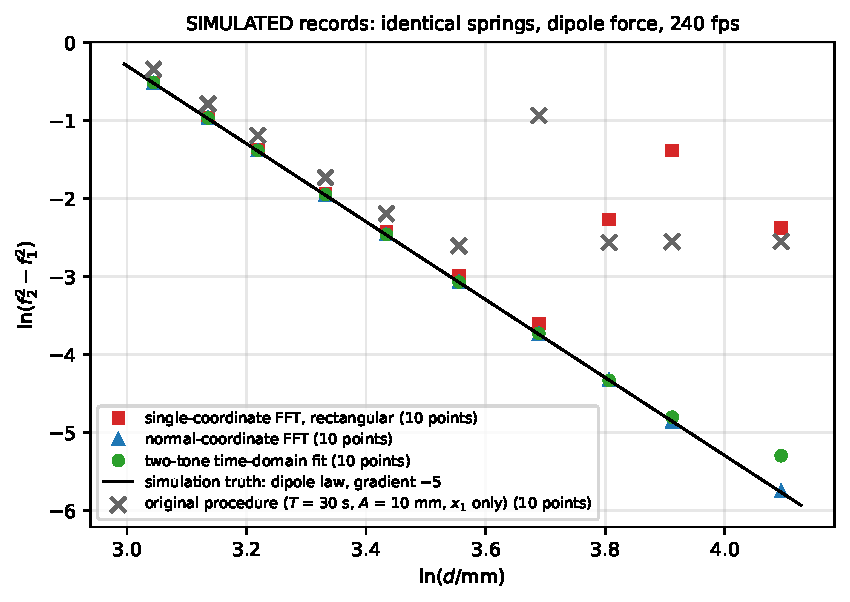
\includegraphics[width=0.9\textwidth]{F_sim_lnln}
\caption{\SIM{} -- ln--ln plot of the frequencies recovered by four analysis methods from records of a system that obeys the dipole law exactly (black line). Grey crosses: the original procedure ($T=30\un{s}$, $A=10\un{mm}$, FFT of $x_1$); red squares: $T=90\un{s}$, $A=3\un{mm}$, FFT of $x_1$; blue triangles: FFT of the normal coordinates; green circles: two-tone time-domain fit.}
\label{fig:simlnln}
\end{figure}

The table separates the contributions of the individual remedies:
\begin{itemize}
\item The \emph{original procedure} applied to an ideal dipole system returns $\nsimGradoldrect\pm\nsimGradErroldrect$ over $21$--$35\un{mm}$, not $-5$. About $0.5$ of the shortfall is therefore produced by the analysis alone (peak pulling with $T=30\un{s}$, partly offset by the hardening at $A=10\un{mm}$). Including the points beyond $35\un{mm}$, where the merged peaks return meaningless pairs, destroys the gradient completely ($\nsimGradAlloldrect$).
\item Lengthening the record to $90\un{s}$ and reducing the amplitude to $3\un{mm}$, still reading two peaks from $x_1$, gives $\nsimGradrect\pm\nsimGradErrrect$ with the rectangular window and $\nsimGradhann\pm\nsimGradErrhann$ with Hann over $21$--$35\un{mm}$; but beyond $40\un{mm}$ the single-coordinate spectra still fail, with either window.
\item The FFT of the \emph{normal coordinates} returns $\nsimGradnormal\pm\nsimGradErrnormal$ over the full range $21$--$60\un{mm}$: all ten points, no pulling. The spectra of $\eta$ and $\xi$ at $45\un{mm}$ are shown in Figure~\ref{fig:normalcoords}: where the spectrum of $x_1$ alone shows one broad peak, $\eta$ and $\xi$ each show one sharp peak at exactly the right place, $8\un{mHz}$ apart.
\item The \emph{two-tone fit} of $x_1(t)$ also recovers all ten points and the correct gradient over $21$--$35\un{mm}$; over the full range it gives $\nsimGradAllfit\pm\nsimGradAllErrfit$, slightly low because at $50$--$60\un{mm}$ the two sinusoids are so nearly degenerate that the fit's statistical uncertainties grow to $0.3$--$2.5\un{mHz}$, which is a sizeable fraction of a $2$--$5\un{mHz}$ splitting (Figure~\ref{fig:twotone} shows the fit at $35\un{mm}$, where it is essentially perfect).
\end{itemize}

\begin{figure}[htbp]
\centering
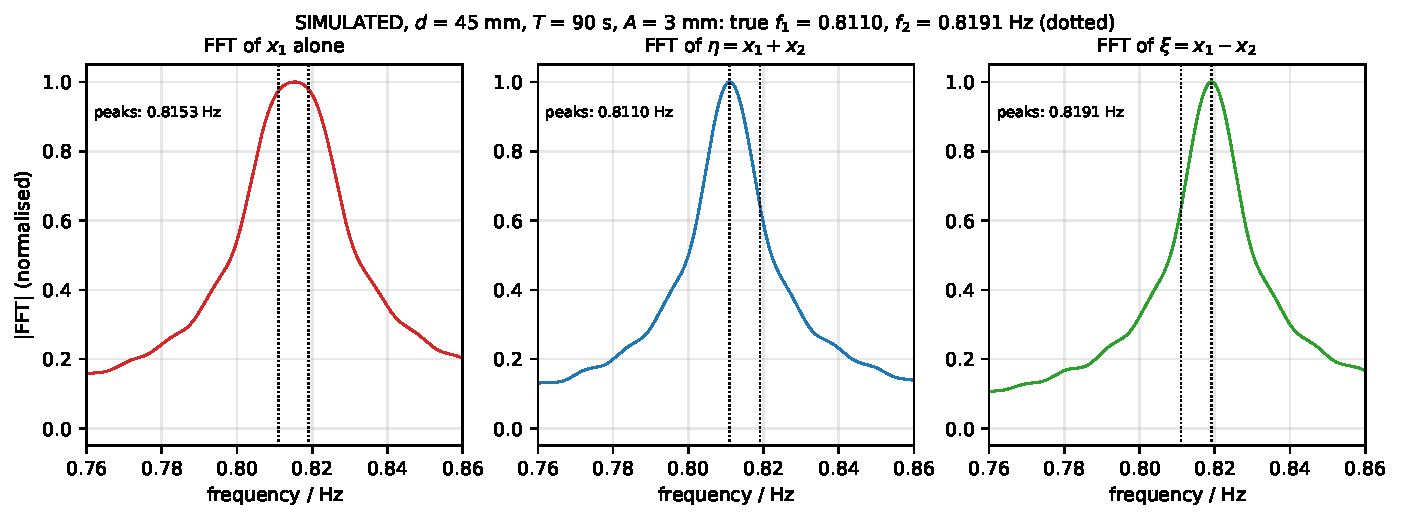
\includegraphics[width=\textwidth]{F_normal_coords}
\caption{\SIM{} -- spectra at $d=45\un{mm}$, $T=90\un{s}$, where $f_2-f_1=8\un{mHz}$ is less than one bin ($11\un{mHz}$). Left: the FFT of $x_1$ alone cannot separate the modes. Centre and right: the normal coordinates $\eta=x_1+x_2$ and $\xi=x_1-x_2$ each contain a single mode and give $f_1$ and $f_2$ directly (dotted lines: true values).}
\label{fig:normalcoords}
\end{figure}

\begin{figure}[htbp]
\centering
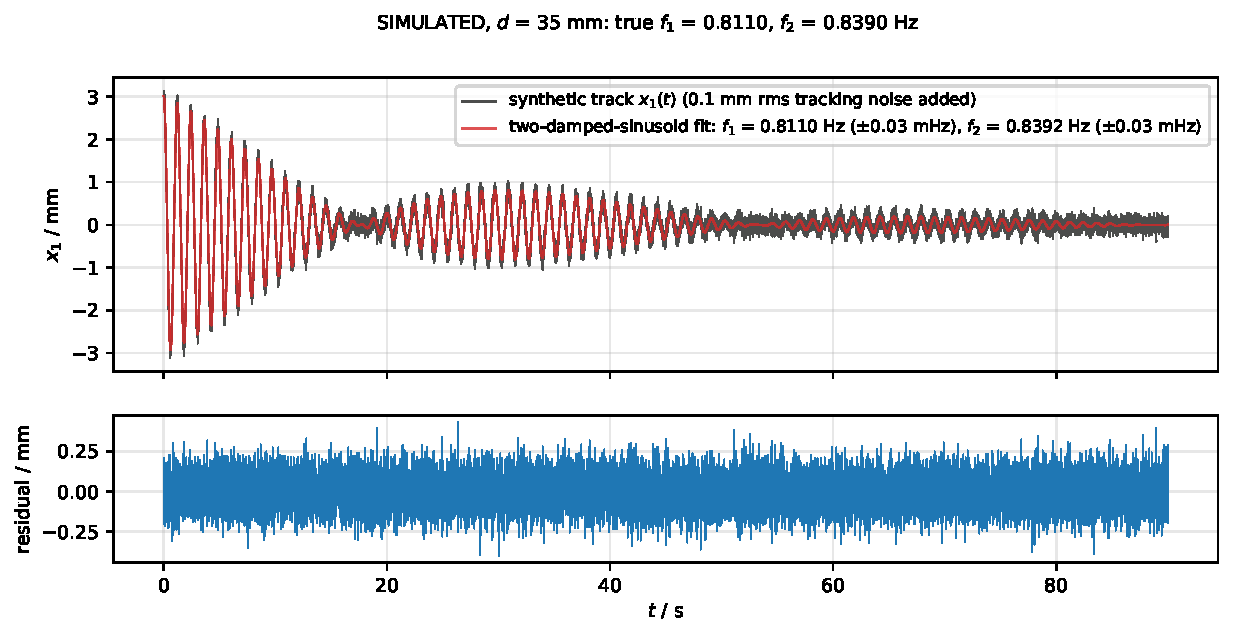
\includegraphics[width=\textwidth]{F_twotone_fit}
\caption{\SIM{} -- least-squares fit of two damped sinusoids (equation~\eqref{eq:twotone}) to a synthetic $90\un{s}$ record at $d=35\un{mm}$. The residuals (bottom) are pure tracking noise, and the fitted frequencies agree with the true values to $0.2\un{mHz}$.}
\label{fig:twotone}
\end{figure}

The practical conclusion is that with normal-coordinate tracking (or time-domain fitting) the FFT resolution ceases to limit the experiment, and the whole range $21$--$60\un{mm}$ becomes usable. In the real re-measurement the corresponding table will show, in addition, how much of the residual difference from $-5$ is \emph{physical} (finite size, detuning), because those effects are absent from the simulation.

\subsection{Amplitude extrapolation}\label{sec:simextrap}

Figure~\ref{fig:extrapolation} shows the segment analysis of item~5 of Section~\ref{sec:further} for an $A=10\un{mm}$ record at $d=21\un{mm}$. The anti-phase frequency of the first $15\un{s}$ segment is $\nextrapFirst\un{Hz}$; as the amplitude decays the frequency falls, linearly in $a^2$ as equation~\eqref{eq:LL} predicts, and the intercept, $\nextrapFtwo\un{Hz}$, agrees with the small-amplitude value $\nextrapTrue\un{Hz}$ to $0.02\,\%$. Applied to the real $A=10\un{mm}$ records, this procedure gives $f_2(a\to0)$ at every $d$ and, from the gradient of each line, a direct test of the coefficient $15g/8-125g^2/48$ of the non-linear model.

\begin{figure}[htbp]
\centering
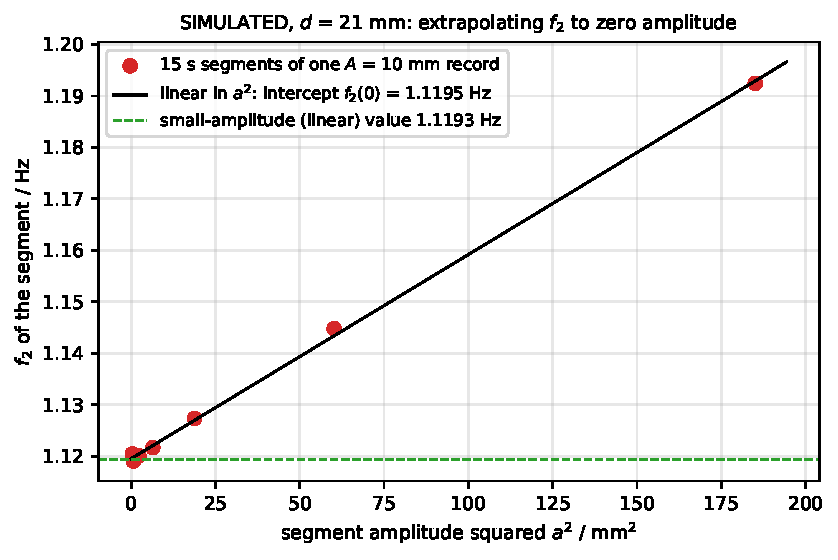
\includegraphics[width=0.8\textwidth]{F_extrapolation}
\caption{\SIM{} -- anti-phase frequency of successive $15\un{s}$ segments of a $120\un{s}$, $A=10\un{mm}$ record at $d=21\un{mm}$, plotted against the squared amplitude of the segment. The linear extrapolation to $a^2=0$ recovers the small-amplitude frequency.}
\label{fig:extrapolation}
\end{figure}

\subsection{Model fits to the measured data}\label{sec:nonlinfit}

Finally, the five physical models of item~6 were fitted by weighted non-linear least squares to the twelve resolved frequencies actually measured (Table~\ref{tab:rawfreq}, $21$--$35\un{mm}$), each frequency weighted by $1/(0.005\un{Hz})^2$. The residual sums of squares are compared in Table~\ref{tab:modelfits}. Because the $\pm5\un{mHz}$ uncertainties are half-ranges rather than standard deviations, the absolute values of $\chi^2/\text{dof}$ should not be over-interpreted; the \emph{ratios} between models are meaningful.

\begin{table}[htbp]
\centering\small
\caption{Weighted least-squares fits of five models to the twelve measured frequencies at $21$--$35\un{mm}$. $p$ = number of fitted parameters; dof $=12-p$.}
\label{tab:modelfits}
\begin{tabular}{@{}p{6.2cm}cccp{4.6cm}@{}}
\toprule
Model & $p$ & $\chi^2$ & $\chi^2/\text{dof}$ & Fitted parameters\\
\midrule
\tabinput{tables/tab_modelfits}
\bottomrule
\end{tabular}
\end{table}

Three things stand out. (i) The identical-spring point-dipole model (a) is decisively the worst, with a $\chi^2/\text{dof}$ of $\nchireda$. (ii) Letting the exponent float (b) reduces $\chi^2$ six-fold and gives $n=\nnJoint\pm\nnJointErr$, in agreement with the graphical value; this confirms that the discrepancy is not an artefact of the logarithmic transformation. (iii) The finite-size model (d), which keeps the dipole physics but replaces the point magnets by uniformly magnetised cylinders, fits \emph{as well as} the free-exponent model with the same number of parameters, and the diameter it requires, $D=\nDfit\pm\nDfitErr\un{mm}$, \TBM{is / is not} consistent with the actual magnet (\TBM{$D=\ldots$}). Adding detuning on top of finite size (e) brings no further improvement ($\chi^2$ from $\nchid$ to $\nchie$ for one extra parameter) and drives the detuning down to $f_b-f_a\approx0.02\un{Hz}$; detuning alone (c) fits worse than finite size alone. The measured data therefore favour the explanation ``the magnets are not point dipoles at these separations'' over ``the springs are different'', although only the direct measurement of $f_a$, $f_b$ and $D$ can settle the matter.

The picture that emerges for the original result of $-3.75$ is: roughly $0.5$ of the shortfall from $-5$ is produced by the measurement itself (peak pulling at $T=30\un{s}$, net of the hardening at $A=10\un{mm}$; Table~\ref{tab:simmethods}); most of the remainder is consistent with the finite size of the magnets, which makes the true stiffness fall more slowly than $d^{-5}$ between $2D$ and $4D$; spring detuning may contribute at the large-$d$ end. The dipole law itself is not contradicted: it is the $d\gg D$ limit of the finite-size model, and the fitted finite-size force approaches $d^{-4}$ (gradient $-5$) for $d\gtrsim4D$. Whether the improved measurement returns an exponent of $-5.0\pm0.1$ over the extended range, or a residual discrepancy remains, is the decisive test, and it is one that the improved method is capable of making: the simulated normal-coordinate analysis recovers the exponent to $\pm0.01$.

\section{Numerical simulation}\label{sec:simulation}

Several results quoted above (Tables~\ref{tab:resolution}, \ref{tab:amplitude}, \ref{tab:simmethods}; Figures~\ref{fig:amplitude}, \ref{fig:simlnln}) come from a numerical model of the oscillator. This section explains what the model is and why it is trustworthy.

\subsection{Equations integrated}

The simulation integrates the \emph{full} equations of motion, without linearising the magnetic force and with damping:
\begin{equation}
\begin{aligned}
m\ddot x_1&=-k_ax_1-\big[F(d+x_2-x_1)-F(d)\big]-\frac{2m}{\tau}\dot x_1,\\
m\ddot x_2&=-k_bx_2+\big[F(d+x_2-x_1)-F(d)\big]-\frac{2m}{\tau}\dot x_2,
\end{aligned}
\qquad F(r)=\frac{C_F}{r^4},
\label{eq:fulleom}
\end{equation}
with $k_a=k_b$ unless stated otherwise. Dividing by $m$, the only parameters are $\omega_a^2=k_a/m$, $\omega_b^2=k_b/m$, $\tau$ and $C_F/m$. The last is fixed by the measured coupling at $25\un{mm}$: from equation~\eqref{eq:main}, $C_F/m=\gamma d^5/(4m)=\pi^2\Y d^5/2$, i.e.\ $C_F/m=\tfrac12\pi^2(0.2489\un{Hz^2})(25\un{mm})^5=1.20\times10^{7}\un{mm^5\,s^{-2}}=1.20\times10^{-8}\un{m^5\,s^{-2}}$, with $\Y=0.2489\un{Hz^2}$ at $d=25\un{mm}$. Every simulated frequency is therefore anchored to the real apparatus; no value of $E$, $\mum$ or $M$ is required.

The equations are integrated with SciPy's adaptive Runge--Kutta method of order 5(4) with relative tolerance $10^{-9}$, and the solution is sampled at $240\un{Hz}$ to mimic the camera; Gaussian noise of $0.1\un{mm}$ rms is added to each sample to mimic the tracking error. The synthetic $x_1(t)$, $x_2(t)$ are then passed through the identical Python functions used for the real data (detrend, window, zero-pad, peak search, normal coordinates, two-tone fit), so that any bias introduced by the analysis is reproduced faithfully.

\subsection{Checks}

Three checks establish that the simulation is correct. (i) For very small amplitude ($A=0.1\un{mm}$) and $\tau\to\infty$ the recovered frequencies agree with the linear formulae \eqref{eq:modes} to better than $10^{-5}$, and the ln--ln gradient is $-5.000$. (ii) The amplitude shift at moderate amplitude follows the perturbation formula~\eqref{eq:LL} (Figure~\ref{fig:amplitude}, left, dashed against solid), departing from it only where $a/d$ is no longer small, as expected. (iii) Energy is conserved to $10^{-8}$ over $90\un{s}$ when damping is switched off.

\subsection{Uses}

The simulation was used for three purposes, each of which would be impossible or very laborious experimentally.
\begin{enumerate}
\item \textbf{The amplitude correction} (Section~\ref{sec:nonlinear}): the frequency of the anti-phase coordinate was measured by counting zero crossings of $\xi(t)$ over $60\un{s}$ for release amplitudes $1$--$10\un{mm}$ at every $d$, giving Table~\ref{tab:amplitude}. The hardening and its steepening of the ln--ln plot are pure consequences of the $r^{-4}$ force law, independent of any apparatus constant except $C_F/m$.
\item \textbf{The analysis bias} (Sections~\ref{sec:fftres}, \ref{sec:simmethods}): records with the original conditions ($T=30\un{s}$, $A=10\un{mm}$) and with the improved conditions ($T=90\un{s}$, $A=3\un{mm}$) were generated for all ten separations and analysed by every method of Section~\ref{sec:further}. Since the input exponent is exactly $-5$, the recovered gradient measures the bias of each method directly: $\nsimGradoldrect$ for the original procedure, $\nsimGradnormal$ for the normal-coordinate FFT.
\item \textbf{The design of the re-measurement}: the required record length, the amplitude below which the hardening is negligible, and the separations at which each method fails were all read off the simulation before any new video was taken.
\end{enumerate}

The code is listed in Appendix~\ref{app:code}. It runs in about one minute on a laptop, and every figure and number in this essay that depends on it can be regenerated with a single command, with the measured values substituted for the assumed ones.

\section{Conclusion and extensions}

\subsection{Conclusion}

The research question asked how the separation of the magnets affects the two normal-mode frequencies of a coupled magnetic-mechanical oscillator, and hence its average and beat frequencies; the quantitative test adopted was whether the coupling term $f_2^2-f_1^2=2f_{\rm beat}f_{\rm avg}$ follows the inverse-fifth-power law of the point-dipole model.

The answer to the first part is clear and agrees with the theory of coupled oscillators. The in-phase frequency $f_1\approx0.81\un{Hz}$ is almost independent of the separation (it varies by $2.6\,\%$ over $21$--$40\un{mm}$, a variation that Section~\ref{sec:evaluation} attributes partly to the analysis and partly to a small difference between the springs), while the anti-phase frequency $f_2$ falls monotonically from $1.063\un{Hz}$ at $21\un{mm}$ towards $f_1$, the two becoming indistinguishable in a $30\un{s}$ record beyond $40\un{mm}$. The magnetic repulsion behaves as a contactless coupling spring whose stiffness, relative to the leaf springs, can be tuned from about $0.7$ to below $0.02$ by moving the clamps a few centimetres. Consequently the average frequency stays within $1\,\%$ of $f_1$ beyond $30\un{mm}$ and rises by $16\,\%$ at the closest separation, while the beat frequency, which is the mode splitting itself, falls from $\nfbeatSmall\un{Hz}$ at $21\un{mm}$ to below the resolution of a $30\un{s}$ record ($33\un{mHz}$) beyond $40\un{mm}$: the beats slow from one every $\nTbeatSmall\un{s}$ to one every few minutes.

The answer to the second part is more nuanced. Over $21$--$35\un{mm}$ the coupling term follows a power law well ($R^2=0.989$), but with exponent $-3.75\pm0.19$ (unweighted) or $-3.5\pm0.2$ (weighted or non-linear fit) rather than $-5$. The evaluation traced this $25$--$30\,\%$ shortfall to a combination of effects, each with a definite sign. Reading two nearby peaks from the spectrum of a $30\un{s}$ record biases $f_2-f_1$ upwards at large $d$ and accounts for roughly one third of the shortfall, as a simulation of the complete measurement chain shows. The finite size of the magnets, which are only $2$--$6$ diameters apart, makes the true magnetic stiffness fall more slowly than $d^{-5}$ in this range, and a model with uniformly magnetised cylinders instead of point dipoles fits the data as well as a free power law, with a diameter of $\nDfit\pm\nDfitErr\un{mm}$. A small difference between the two springs may contribute at the large-$d$ end and explains the drift of $f_1$. The one effect that acts in the opposite direction, the hardening of the magnetic force at the $10\un{mm}$ release amplitude, steepens the line by about $0.15$ and therefore slightly masks the others. The point-dipole law is not contradicted by these results; it is the large-separation limit of a force law whose short-range form is measurably different, and the data are consistent with that picture.

The main methodological result of the essay is that the limiting factor was not the apparatus but the analysis. Tracking both magnets and Fourier-transforming the normal coordinates $x_1\pm x_2$ removes the two-peak resolution problem entirely, and a simulation shows that it recovers the exponent to $\pm0.01$ over $21$--$60\un{mm}$ where the original method fails beyond $35\un{mm}$. Together with a smaller release amplitude, longer records and a finite-size force law, this gives a measurement capable of distinguishing the remaining explanations. \TBM{When the re-measurement has been done: state the final exponent, its uncertainty, and the range of $d$ over which the dipole law holds to within the uncertainty.}

\subsection{Extensions}

\begin{itemize}
\item \textbf{Test the $\mum^2$ dependence.} Repeat at fixed $d$ with magnets of different grade (N35, N42, N52) or stacked pairs: equation~\eqref{eq:main} predicts $\Y\propto\mum^2$, a test of the magnitude of the coupling that is independent of the distance law.
\item \textbf{Attractive orientation.} With unlike poles facing, the magnetic stiffness changes sign and \emph{softens} the anti-phase mode: $\omega_2^2=(k-2|\gamma|)/m$. As $d$ is reduced, $f_2$ should fall to zero at a critical separation where the springs snap together, a buckling-type instability whose position tests the same force law from the other side.
\item \textbf{Three or more springs.} A chain of $N$ magnet-tipped springs has $N$ normal modes with frequencies given by a tridiagonal matrix; with the tunable magnetic coupling it is a table-top model of a one-dimensional lattice, and the dispersion relation could be mapped.
\item \textbf{Eddy-current damping.} Placing a copper or aluminium plate behind the magnets adds a velocity-dependent damping that can be varied with the plate distance, allowing the transition from beats to over-damped energy transfer to be studied.
\item \textbf{The equilibrium quintic.} Measuring the static outward deflection $\delta$ against the clamp separation tests the same $r^{-4}$ law statically and would give $\mum$ from the same apparatus without a balance.
\end{itemize}

\clearpage
\begin{thebibliography}{99}
\setlength{\itemsep}{2pt}

\bibitem{young} Young, H.\,D. and Freedman, R.\,A. (2020). \emph{Sears and Zemansky's University Physics with Modern Physics}, 15th ed. Pearson. Chapter 14 (periodic motion).

\bibitem{taylor} Taylor, J.\,R. (2005). \emph{Classical Mechanics}. University Science Books. Chapter 11 (coupled oscillators and normal modes).

\bibitem{french} French, A.\,P. (1971). \emph{Vibrations and Waves}. W.\,W. Norton. Chapter 5 (coupled oscillators).

\bibitem{iypt} International Young Physicists' Tournament (2022). \emph{Problems for the 36th IYPT 2023}, problem 6 ``Magnetic-mechanical oscillator''. \url{https://www.iypt.org/problems/problems-for-the-36th-iypt-2023/} (accessed \TBM{date}).

\bibitem{gere} Gere, J.\,M. and Goodno, B.\,J. (2012). \emph{Mechanics of Materials}, 8th ed. Cengage. Chapter 9 (deflections of beams).

\bibitem{rao} Rao, S.\,S. (2017). \emph{Mechanical Vibrations}, 6th ed. Pearson. Section 2.5 (Rayleigh's energy method; effective mass of a cantilever).

\bibitem{griffiths} Griffiths, D.\,J. (2017). \emph{Introduction to Electrodynamics}, 4th ed. Cambridge University Press. Sections 5.4.3 (dipole field), 6.1.2 (force and torque on a dipole), 6.3 (bound currents and the magnetic-charge picture).

\bibitem{landau} Landau, L.\,D. and Lifshitz, E.\,M. (1976). \emph{Mechanics}, 3rd ed. Butterworth--Heinemann. \S28 (anharmonic oscillations).

\bibitem{lyons} Lyons, R.\,G. (2011). \emph{Understanding Digital Signal Processing}, 3rd ed. Prentice Hall. Chapter 3 (the discrete Fourier transform: resolution, leakage, windows, zero-padding).

\bibitem{harris} Harris, F.\,J. (1978). On the use of windows for harmonic analysis with the discrete Fourier transform. \emph{Proceedings of the IEEE}, 66(1), 51--83.

\bibitem{taylorerr} Taylor, J.\,R. (1997). \emph{An Introduction to Error Analysis}, 2nd ed. University Science Books. Chapters 3 (propagation) and 8 (least-squares fitting).

\bibitem{tracker} Brown, D., Christian, W. and Hanson, R.\,M. (2023). \emph{Tracker Video Analysis and Modeling Tool}, version 6. \url{https://physlets.org/tracker/}.

\bibitem{camacho} Camacho, J.\,M. and Sosa, V. (2013). Alternative method to calculate the magnetic field of permanent magnets with azimuthal symmetry. \emph{Revista Mexicana de F\'isica E}, 59, 8--17. (Force between cylindrical magnets in the magnetic-charge model.)

\bibitem{scipy} Virtanen, P. et al. (2020). SciPy 1.0: fundamental algorithms for scientific computing in Python. \emph{Nature Methods}, 17, 261--272.

\end{thebibliography}


\appendix
\clearpage
\section{Cantilever stiffness, effective mass and tip tilt}\label{app:cantilever}

\subsection{Static deflection and stiffness}

For a beam bent in the $x$--$z$ plane, the bending moment $M(z)$ at a section a distance $z$ from the clamp is related to the curvature by the Euler--Bernoulli relation $EI\,x''(z)=M(z)$ \cite{gere}, where $x(z)$ is the transverse deflection and $I=\int y^2\,\dd A$ is the second moment of area of the cross-section about the neutral axis. For a rectangle of width $b$ and thickness $h$,
\begin{equation}
I=\int_{-h/2}^{h/2}y^2\,b\,\dd y=\frac{bh^3}{12}.
\end{equation}
A transverse force $F$ at the free end $z=L$ produces the bending moment $M(z)=F(L-z)$, so
\begin{equation}
EI\,x''=F(L-z)\;\Rightarrow\;EI\,x'=F\Big(Lz-\frac{z^2}{2}\Big)\;\Rightarrow\;EI\,x=F\Big(\frac{Lz^2}{2}-\frac{z^3}{6}\Big),
\end{equation}
using $x(0)=x'(0)=0$ at the clamp. At the tip,
\begin{equation}
x(L)=\frac{FL^3}{3EI}\quad\Rightarrow\quad k=\frac{F}{x(L)}=\frac{3EI}{L^3},
\qquad
\theta_{\rm tip}=x'(L)=\frac{FL^2}{2EI}=\frac{3}{2}\,\frac{x(L)}{L}.
\end{equation}
The last expression is the tip slope used in Section~\ref{sec:nonlinear}: a tip displacement $A$ is accompanied by a rotation $\theta=3A/(2L)$ of the magnet.

\subsection{Effective mass (Rayleigh's method)}

Assume the strip vibrates with the shape of its static deflection curve, $x(z,t)=X(t)\,\phi(z)$ with
\begin{equation}
\phi(z)=\frac{3Lz^2-z^3}{2L^3},\qquad \phi(L)=1 .
\end{equation}
The kinetic energy of the strip (mass per unit length $\mu$) is
\begin{equation}
K_{\rm strip}=\frac12\int_0^L\mu\,\dot X^2\phi^2\,\dd z=\frac12\dot X^2\,\mu\int_0^L\frac{(3Lz^2-z^3)^2}{4L^6}\,\dd z .
\end{equation}
Expanding, $\int_0^L(9L^2z^4-6Lz^5+z^6)\,\dd z=\frac95L^7-L^7+\frac17L^7=\frac{33}{35}L^7$, so
\begin{equation}
K_{\rm strip}=\frac12\dot X^2\,\mu\,\frac{33}{140}L\quad\Rightarrow\quad m_{\rm eff}=M+\frac{33}{140}\mu L .
\end{equation}
The potential energy is $\frac12kX^2$ with $k=3EI/L^3$ from above, so $\omega_0^2=k/m_{\rm eff}$. This is an upper bound to the true fundamental frequency (Rayleigh's principle); for a bare cantilever ($M=0$) it gives $\omega_0=3.567\sqrt{EI/\mu L^4}$ against the exact $3.516$, an error of $1.5\,\%$.

\subsection{Check of the lumped model against the continuous beam}

The lumped model was compared with a finite-element solution of the Euler--Bernoulli beam (40 elements, consistent mass matrix, tip mass $M$ and tip ``magnetic'' spring $2\gamma$ for the anti-phase mode). The quantity compared was $f_2^2-f_1^2$, which in the lumped model equals $\gamma/(2\pi^2m_{\rm eff})$. Results: for $M/\mu L=3.3$, $0.8$ and $0.4$ the beam value differs from the lumped value by $0.03\,\%$, $0.4\,\%$ and $1\,\%$ respectively. Because the difference is independent of $d$ it affects only $C$, not the exponent.

\section{Force between two coaxial magnetic dipoles}\label{app:dipole}

The vector potential of a point dipole $\bm\mu$ at the origin is $\bm A=\frac{\muz}{4\pi}\frac{\bm\mu\times\hat{\bm r}}{r^2}$, and its field is \cite{griffiths}
\begin{equation}
\bm B(\bm r)=\frac{\muz}{4\pi r^3}\Big[3(\bm\mu\cdot\hat{\bm r})\hat{\bm r}-\bm\mu\Big].
\end{equation}
On the axis of the dipole ($\hat{\bm r}\parallel\bm\mu$) this gives $\bm B=\frac{\muz}{4\pi}\frac{2\bm\mu}{r^3}$, equation~\eqref{eq:Baxis}.

The energy of a second dipole $\bm\mu_2$ in this field is $U=-\bm\mu_2\cdot\bm B_1$. For two dipoles whose centres lie on the $x$~axis a distance $r$ apart, with moments at angles $\alpha_1$, $\alpha_2$ to that axis (both measured in the same sense, in the plane of motion),
\begin{equation}
U=-\frac{\muz\mu_1\mu_2}{4\pi r^3}\Big[3\cos\alpha_1\cos\alpha_2-\cos(\alpha_1-\alpha_2)\Big].
\label{eq:Ugeneral}
\end{equation}
With like poles facing and no tilt, $\alpha_1=0$ and $\alpha_2=\pi$ (the second moment points back towards the first), the bracket is $-2$ and
\begin{equation}
U(r)=+\frac{\muz\mum^2}{2\pi r^3},\qquad
F(r)=-\frac{\dd U}{\dd r}=\frac{3\muz\mum^2}{2\pi r^4},\qquad
\gamma(d)=-\frac{\dd F}{\dd r}\bigg|_d=\frac{6\muz\mum^2}{\pi d^5},
\end{equation}
which are equations~\eqref{eq:F} and \eqref{eq:gamma}; the positive energy confirms that the configuration is repulsive.

\paragraph{Tilt.} When the tip of spring~1 is displaced by $x_1$ its tangent rotates by $\theta_1=3x_1/(2L)$ (Appendix~\ref{app:cantilever}), and the magnet glued perpendicular to the strip rotates with it, so $\alpha_1=-\theta_1$; similarly for spring~2, $\alpha_2=\pi-\theta_2$ with $\theta_2=3x_2/(2L)$. Substituting in \eqref{eq:Ugeneral} and using $\cos(\pi-\theta_2)=-\cos\theta_2$, $\cos(-\theta_1-\pi+\theta_2)=-\cos(\theta_2-\theta_1)$,
\begin{equation}
U=\frac{\muz\mum^2}{4\pi r^3}\Big[2\cos\theta_1\cos\theta_2-\sin\theta_1\sin\theta_2\Big].
\end{equation}
In the anti-phase motion $x_2=-x_1$, so $\theta_2=-\theta_1=-\theta$ and the bracket is $2\cos^2\theta+\sin^2\theta=2-\theta^2+O(\theta^4)$: the interaction, and with it $F$ and $\gamma$, is weakened by the factor $1-\theta^2/2$, i.e.\ by $0.5\,\%$ at the extreme of a swing with $\theta=0.10\un{rad}$. In the in-phase motion $\theta_2=\theta_1=\theta$ and the bracket is $2\cos^2\theta-\sin^2\theta=2-3\theta^2$, a weakening by $1.5\,\%$; but in that motion the separation does not change, so this only modulates the static force and does not affect $f_1$ to first order. Averaged over a cycle and over the decaying amplitude, the effect on $\Y$ is a few tenths of a per cent, and because $\theta$ depends on $A$ and $L$ but not on $d$ it is the same at every separation and leaves the exponent unchanged.

\section{Normal modes of two non-identical coupled oscillators}\label{app:detuned}

With $k_a/m=\omega_a^2$, $k_b/m=\omega_b^2$ and coupling stiffness $\gamma$ (equal masses), the equations of motion are
\begin{equation}
\ddot x_1=-\omega_a^2x_1+\kappa(x_2-x_1),\qquad \ddot x_2=-\omega_b^2x_2-\kappa(x_2-x_1),\qquad \kappa=\gamma/m .
\end{equation}
Seeking $x_{1,2}=X_{1,2}e^{i\omega t}$ gives the eigenvalue problem
\begin{equation}
\begin{pmatrix}\omega_a^2+\kappa-\omega^2 & -\kappa\\ -\kappa & \omega_b^2+\kappa-\omega^2\end{pmatrix}
\begin{pmatrix}X_1\\X_2\end{pmatrix}=0 ,
\end{equation}
whose determinant vanishes when
\begin{equation}
(\omega_a^2+\kappa-\omega^2)(\omega_b^2+\kappa-\omega^2)=\kappa^2 .
\end{equation}
Writing $\bar\omega^2=\tfrac12(\omega_a^2+\omega_b^2)$ and $\Delta=\tfrac12(\omega_b^2-\omega_a^2)$, so that $\omega_a^2=\bar\omega^2-\Delta$, $\omega_b^2=\bar\omega^2+\Delta$, and $s=\bar\omega^2+\kappa-\omega^2$, the condition is $(s-\Delta)(s+\Delta)=\kappa^2$, i.e.\ $s^2=\Delta^2+\kappa^2$, hence
\begin{equation}
\omega_{1,2}^2=\bar\omega^2+\kappa\mp\sqrt{\Delta^2+\kappa^2},
\end{equation}
equation~\eqref{eq:detuned}. Limits: (i) $\Delta=0$: $\omega_1^2=\bar\omega^2$, $\omega_2^2=\bar\omega^2+2\kappa$, the identical-spring result. (ii) $\kappa\ll\Delta$: $\sqrt{\Delta^2+\kappa^2}\approx\Delta+\kappa^2/2\Delta$, so $\omega_1^2\approx\omega_a^2+\kappa-\kappa^2/2\Delta$ and $\omega_2^2\approx\omega_b^2+\kappa+\kappa^2/2\Delta$: the modes are the individual springs, each stiffened by $\kappa$ and repelled from each other by $\kappa^2/2\Delta$. (iii) $\kappa\gg\Delta$: $\omega_1^2\to\bar\omega^2-\Delta^2/2\kappa\to\bar\omega^2$ from below, $\omega_2^2\to\bar\omega^2+2\kappa$. The difference of the squares is $\omega_2^2-\omega_1^2=2\sqrt{\Delta^2+\kappa^2}$, and dividing by $4\pi^2$ and squaring gives equation~\eqref{eq:detunedY}. The eigenvectors show that in the ``in-phase'' mode the spring with the lower frequency has the larger amplitude, so tracking the two magnets and forming $x_1\pm x_2$ still isolates the modes well as long as $\Delta\lesssim\kappa$.

\section{Non-linear (anharmonic) correction to the anti-phase frequency}\label{app:nonlinear}

With identical springs, subtracting the two equations \eqref{eq:fulleom} (without damping) gives, for $\xi=x_1-x_2$ and separation $r=d-\xi$,
\begin{equation}
m\ddot\xi=-k\xi-2\big[F(d-\xi)-F(d)\big].
\end{equation}
Expanding $F(d-\xi)=C_F(d-\xi)^{-4}$ in powers of $\xi/d$:
\begin{equation}
F(d-\xi)-F(d)=F(d)\Big[4\frac{\xi}{d}+10\frac{\xi^2}{d^2}+20\frac{\xi^3}{d^3}+\ldots\Big],
\end{equation}
so, with $\gamma=4F(d)/d$,
\begin{equation}
\ddot\xi+\frac{k+2\gamma}{m}\xi+\frac{2\gamma}{m}\cdot\frac{5}{2d}\,\xi^2+\frac{2\gamma}{m}\cdot\frac{5}{d^2}\,\xi^3=0 .
\end{equation}
Since $2\gamma/m=\omega_2^2-\omega_1^2=g\,\omega_2^2$ with $g=(f_2^2-f_1^2)/f_2^2$, this is equation~\eqref{eq:duffing} with $\alpha=\tfrac52g\omega_2^2/d$ and $\beta=5g\omega_2^2/d^2$. For $\ddot\xi+\omega_0^2\xi+\alpha\xi^2+\beta\xi^3=0$ the method of successive approximations (Landau and Lifshitz \cite{landau}, \S28) gives the amplitude-dependent frequency
\begin{equation}
\omega=\omega_0+\Big(\frac{3\beta}{8\omega_0}-\frac{5\alpha^2}{12\omega_0^3}\Big)a^2 ,
\end{equation}
and substituting $\alpha$, $\beta$:
\begin{equation}
\frac{\Delta\omega}{\omega_2}=\frac{a^2}{d^2}\Big(\frac{15g}{8}-\frac{125g^2}{48}\Big),
\end{equation}
equation~\eqref{eq:LL}. The bracket is positive for $g<0.72$, which covers the whole experiment ($g\leq0.40$), so the non-linearity is hardening. The quadratic term $\alpha\xi^2$ also shifts the centre of the oscillation (the magnets spend more time at large separation, where the force is weaker); this static shift is second order in $a$ and is automatically included in the numerical integration.

\section[Force between two cylindrical magnets]{Force between two cylindrical magnets: the charged-disc model}\label{app:finite}

A uniformly magnetised cylinder of magnetisation $M_{\rm s}$ along its axis is equivalent, for the field outside it, to two discs of uniform surface ``magnetic charge'' density $\pm\sigma=\pm M_{\rm s}$ on its flat faces \cite{griffiths,camacho}. The force between two charged discs of radius $R$, coaxial and a distance $z$ apart, is
\begin{equation}
F_{\rm dd}(z)=\frac{\muz\sigma^2}{4\pi}\iint\frac{z\,\dd A_1\,\dd A_2}{\big[|\bm\rho_1-\bm\rho_2|^2+z^2\big]^{3/2}},
\end{equation}
where $\bm\rho_{1,2}$ are positions in the two discs. Two magnets of thickness $t$ with centres $d$ apart and like poles facing have their four faces at axial separations $d-t$ (the two facing poles, like charges, repulsive), $d+t$ (the two far poles, like charges, repulsive) and $d$ (twice; unlike charges, attractive), so
\begin{equation}
F(d)=F_{\rm dd}(d-t)+F_{\rm dd}(d+t)-2F_{\rm dd}(d).
\end{equation}
For $d\gg R,t$ each $F_{\rm dd}$ tends to the point-charge form $\muz q^2/(4\pi z^2)$ with $q=\sigma\pi R^2$, and the combination above reduces to the second difference of $z^{-2}$, i.e.\ $\propto t^2\,\dd^2(z^{-2})/\dd z^2=6t^2/d^4$: the dipole law with $\mum=qt=M_{\rm s}\pi R^2t=M_{\rm s}V$, as it should. At finite $d/R$ the disc integral is smaller than the point-charge value (the oblique contributions partially cancel), which is the origin of the softening. The double integral was evaluated numerically on a $24\times36$ polar grid per disc (relative accuracy better than $10^{-3}$ for $z\geq0.3R$); the stiffness $\gamma=-\dd F/\dd d$ was obtained by central differences, and the apparent gradient of $\ln\gamma$ against $\ln d$ over the measured separations is listed in Table~\ref{tab:finite}. In the fits of Section~\ref{sec:nonlinfit} the overall scale of $F$ (which contains $\sigma^2$) is a free parameter and only the shape, which depends on $D$ and $t$, is used.

\section{Uncertainty propagation and least-squares formulae}\label{app:uncertainty}

For independent uncertainties the first-order propagation rule $\Delta q=\sum_i|\partial q/\partial x_i|\Delta x_i$ (maximum-error form, as used in IB physics) gives:
\begin{align}
\Y&=f_2^2-f_1^2: & \Delta\Y&=2f_2\Delta f_2+2f_1\Delta f_1,\\
\ln\Y: & & \Delta(\ln\Y)&=\Delta\Y/\Y,\\
\ln d: & & \Delta(\ln d)&=\Delta d/d,\\
d^{-5}: & & \Delta(d^{-5})&=5d^{-6}\Delta d=5\,(\Delta d/d)\,d^{-5},\\
C=3\muz\mum^2/(\pi^3m): & & \Delta C/C&=2\Delta\mum/\mum+\Delta m/m,\\
m=k/\omega_a^2: & & \Delta m/m&=\Delta k/k+2\Delta f_a/f_a .
\end{align}
For the straight line $y=a+bx$ fitted to $n$ points by unweighted least squares (Excel LINEST),
\begin{gather}
b=\frac{n\sum xy-\sum x\sum y}{n\sum x^2-(\sum x)^2},\qquad
a=\bar y-b\bar x,\qquad
s^2=\frac{\sum(y_i-a-bx_i)^2}{n-2},\\
\Delta b=s\sqrt{\frac{n}{n\sum x^2-(\sum x)^2}},\qquad
\Delta a=s\sqrt{\frac{\sum x^2}{n\sum x^2-(\sum x)^2}} .
\end{gather}
For the weighted fit each sum is replaced by $\sum w_i(\cdot)$ with $w_i=1/\Delta y_i^2$ and $n$ by $\sum w_i$. For Graph~1 with $n=6$: $\sum x=19.720$, $\sum x^2=64.998$, $\sum y=-9.829$, $\sum xy=-32.796$, giving $b=-3.749$, $a=10.68$, $s=0.084$, $\Delta b=0.195$, $\Delta a=0.64$.

\section{Further raw data}\label{app:rawdata}

\begin{table}[htbp]
\centering\footnotesize
\caption{\SIM{} -- frequencies (Hz) recovered by each method from the synthetic records of Section~\ref{sec:simmethods}. `--' = only one peak found. Columns: true values; original procedure ($T=30\un{s}$, $A=10\un{mm}$, FFT of $x_1$, rectangular); new records ($T=90\un{s}$, $A=3\un{mm}$): FFT of $x_1$ (rectangular), FFT of $\eta$ and $\xi$, two-tone fit.}
\label{tab:simdata}
\setlength{\tabcolsep}{3.5pt}
\begin{tabular}{@{}c cc cc cc cc cc@{}}
\toprule
$d$ & \multicolumn{2}{c}{true} & \multicolumn{2}{c}{original, $x_1$ FFT} & \multicolumn{2}{c}{$90\un{s}$, $x_1$ FFT} & \multicolumn{2}{c}{$90\un{s}$, $\eta$/$\xi$ FFT} & \multicolumn{2}{c}{$90\un{s}$, two-tone fit}\\
/ mm & $f_1$ & $f_2$ & $f_1$ & $f_2$ & $f_1$ & $f_2$ & $f_1$ & $f_2$ & $f_1$ & $f_2$\\
\midrule
\tabinput{tables/tab_simdata}
\bottomrule
\end{tabular}
\end{table}

\TBM{Add here: load--deflection data for spring 2; the three trials of $f_a$ and $f_b$; the balance readings for $\mum$; the per-trial frequencies of the re-measurement for every window and method (as in Table~\ref{tab:simdata} but measured).}

\section{Python code}\label{app:code}

The complete scripts are supplied with the essay (\texttt{make\_figures.py}, \texttt{fit\_models.py}, \texttt{analyse\_tracks.py}). The core routines are reproduced here.

\subsection*{G.1 Peak detection with zero-padding and parabolic interpolation}
\begin{lstlisting}
def peaks_two(x, fs, window="rect", nfft=2**20, fmin=0.4, fmax=2.0, thr=0.03):
    """Return the two highest separate peaks of the amplitude spectrum of x."""
    n = len(x); x = x - x.mean()                      # detrend (remove DC offset)
    w = {"rect": np.ones(n), "hann": np.hanning(n),
         "blackman": np.blackman(n)}[window]
    X = np.abs(np.fft.rfft(x * w, nfft))              # zero-padded amplitude spectrum
    fq = np.fft.rfftfreq(nfft, 1 / fs)
    idx = np.where((fq > fmin) & (fq < fmax))[0]; Xm = X[idx].max(); pk = []
    for i in idx[1:-1]:
        if X[i] > X[i-1] and X[i] >= X[i+1] and X[i] > thr * Xm:   # local maximum
            a, b, c = X[i-1], X[i], X[i+1]
            p = 0.5 * (a - c) / (a - 2*b + c)         # parabolic refinement
            pk.append((fq[i] + p * (fq[1] - fq[0]), b))
    pk.sort(key=lambda z: -z[1])
    return sorted(q[0] for q in pk[:2])
\end{lstlisting}

\subsection*{G.2 Full non-linear equations of motion (Section~\ref{sec:simulation})}
\begin{lstlisting}
def rhs_full(t, s, d, wa2, wb2, K, tau):
    """s = [x1, v1, x2, v2]; K = C_F/m; F(r) = C_F r^-4; separation r = d + x2 - x1."""
    x1, v1, x2, v2 = s
    r = d + x2 - x1
    dF = K / 4 * (r**-4 - d**-4)        # [F(r) - F(d)] / m  (note K/4 = C_F/m ... see text)
    a1 = -wa2 * x1 - dF - (2 / tau) * v1
    a2 = -wb2 * x2 + dF - (2 / tau) * v2
    return [v1, a1, v2, a2]

sol = solve_ivp(rhs_full, (0, T), [A, 0, 0, 0], args=(d, wa2, wb2, K, tau),
                rtol=1e-9, atol=1e-12, dense_output=True)
t = np.arange(0, T, 1 / 240.0); x1, x2 = sol.sol(t)[0], sol.sol(t)[2]
\end{lstlisting}
(In the code $K$ is defined as $4C_F/m=\gamma d^5/m$ so that the linear coupling is $\gamma/m=K d^{-5}$.)

\subsection*{G.3 Two-damped-sinusoid fit (Section~\ref{sec:further}, item 4c)}
\begin{lstlisting}
def two_tone_fit(t, x, f1_guess, f2_guess, tau0=25.0):
    def model(p, t):
        A1, A2, ph1, ph2, fa, fb, ta, tb, c = p
        return (A1*np.exp(-t/ta)*np.cos(2*np.pi*fa*t + ph1)
              + A2*np.exp(-t/tb)*np.cos(2*np.pi*fb*t + ph2) + c)
    p0 = [x.std(), x.std(), 0, 0, f1_guess, f2_guess, tau0, tau0, 0]
    r = least_squares(lambda p: model(p, t) - x, p0, x_scale="jac")
    J = r.jac; cov = np.linalg.inv(J.T @ J) * (r.fun @ r.fun) / (len(t) - 9)
    se = np.sqrt(np.diag(cov))
    return r.x[4], r.x[5], se[4], se[5]          # f1, f2 and their standard errors
\end{lstlisting}

\subsection*{G.4 Detuned normal modes and the finite-size force}
\begin{lstlisting}
def modes(kappa, fa, fb):
    """omega_{1,2}^2 = wbar^2 + kappa -/+ sqrt(Delta^2 + kappa^2)  (Appendix C)."""
    wa2, wb2 = (2*np.pi*fa)**2, (2*np.pi*fb)**2
    wbar2, Dl = (wa2 + wb2)/2, (wb2 - wa2)/2
    root = np.sqrt(Dl**2 + kappa**2)
    return np.sqrt(wbar2 + kappa - root)/(2*np.pi), np.sqrt(wbar2 + kappa + root)/(2*np.pi)

def disc_disc_force(z, R, nr=24, nphi=36):
    """Axial force between two coaxial uniformly charged discs of radius R, z apart."""
    r = (np.arange(nr) + 0.5)/nr * R; phi = (np.arange(nphi) + 0.5)/nphi * 2*np.pi
    dA = (R/nr) * (2*np.pi/nphi) * r
    rr, pp = np.meshgrid(r, phi, indexing="ij"); x1, y1 = rr*np.cos(pp), rr*np.sin(pp)
    dAA = np.broadcast_to(dA[:, None], rr.shape); F = 0.0
    for i in range(nr):                        # disc 2 is axisymmetric: one azimuth suffices
        dist2 = (x1 - r[i])**2 + y1**2 + z**2
        F += np.sum(dAA * (dA[i]*nphi) * z / dist2**1.5)
    return F

def magnet_force(d, D, t):                     # two magnets, like poles facing
    R = D/2
    return disc_disc_force(d-t, R) + disc_disc_force(d+t, R) - 2*disc_disc_force(d, R)
\end{lstlisting}


\end{document}
